% ########################################

\chapter{On-Site Commissioning}
\label{chap:commissioning}

% ~~~~~~~~~~~~~~~~~~~~

\chaptoc{}

% ########################################

\section{Introduction}
\label{sec:commissioning_intro}

% ~~~~~~~~~~~~~~~~~~~~

\begin{colsection}

In this chapter I describe commissioning the GOTO hardware and parallel software developments.
%
\begin{itemize}
    \item In \nref{sec:hardware_commissioning} I give an outline of the commissioning period, focusing on my own involvement with trips to La Palma and building additional hardware for the dome.
    \item In \nref{sec:software_commissioning} I describe how the control software was developed alongside the hardware, including creating nightly observing routines to take flat fields and focus the telescopes, and how challenges arising from hardware issues were overcome.
\end{itemize}
%
All work described in this chapter is my own unless otherwise indicated, and has not been published elsewhere. Commissioning the GOTO hardware on La Palma was carried out along with several members of the GOTO collaboration; in particular Vik Dhillon and Stu Littlefair from Sheffield; Danny Steeghs, Krzysztof Ulaczyk and Paul Chote from Warwick; Kendall Ackley from Monash; and several undergraduate and postgraduate students from the GOTO member institutions.

\end{colsection}

% ########################################

\section{Deploying the hardware}
\label{sec:hardware_commissioning}

% ~~~~~~~~~~~~~~~~~~~~

\begin{colsection}

GOTO commissioning began with the installation of the prototype telescope on La Palma in the spring of 2017. Over 2017 and 2018 I spent a total of nine weeks on-site, helping deploy the hardware as well as commissioning and developing the G-TeCS software described in previous chapters.

\end{colsection}

% ~~~~~~~~~~~~~~~~~~~~

\subsection{Deployment timeline}
\label{sec:timeline}
\begin{colsection}

GOTO was envisioned as a quick, simple and cheap project that could provide a large field of view to cover the early gravitational-wave skymaps produced by LIGO.\@ When I first interviewed to join the project in February 2015 it was anticipated that GOTO would be up and running imminently, perhaps before the end of that year. Ultimately that did not happen, as can be seen in the project timeline given in \aref{tab:timeline}, and GOTO did not see first light until June 2017. In hindsight the delay was irrelevant, as the first (and, at the time of writing, only) gravitational-wave event to have an electromagnetic counterpart occurred two months later in August 2017 --- and was only visible from the southern hemisphere \citep{GW170817,GW170817_followup}.

GOTO's deployment date was repeatedly set back for a variety of reasons, including planning permission being held up by local tax disputes and delays in manufacturing the mount and optics. The site was ready months before the telescope was, with the first dome being built in November 2016. My first visit to La Palma took place in March 2017, while the telescopes and mount were still in the factory. Vik Dhillon and I went out to the site to develop the dome control and conditions monitoring systems as described in \aref{sec:dome} and \aref{sec:conditions}. During this trip we also installed the additional dome hardware systems I had built, which are described in \aref{sec:arduino}.

\begin{figure}[p]
    \begin{center}
        \begin{tabular}{cl|@{\tls}l} %chktex 44
            2015 & July      & Collaboration meeting in Warwick (29 Jul) \\
                 &           & Site planning application submitted \\
                 & September & Research collaboration agreement signed \\
                 &           & \textit{LIGO's first observing run (O1) begins} \\
                 &           & \textit{First observation of gravitational waves (GW150914)} \\
            \midrule
            2016 & January   & \textit{O1 ends} \\
                 & August    & Planning permission granted \\
                 & September & Site construction begins \\
                 & November  & First dome assembled \\
                 &           & \textit{LIGO's second observing run (O2) begins} \\
            \midrule
            2017 & March     & \textcolor{Blue}{Trip 1 (23--31 Mar) --- install dome systems} \\
                 & May       & Telescope hardware shipped \\
                 & June      & \textbf{GOTO first light (10 Jun)} \\
                 &           & Collaboration meeting in Warwick (19--20 Jun) \\
                 &           & \textcolor{Blue}{Trip 2 (22 Jun--7 Jul) --- install control software} \\
                 & July      & Inauguration ceremony (3 July) \\
                 &           & Dec axis encoder fails \\
                 &           & \textcolor{Blue}{Trip 3 (20--28 Jul) --- pilot commissioning} \\
                 &           & Robotic operations begin \\
                 & August    & UT3 mirrors sent back to manufactures \\
                 &           & \textit{Virgo joins O2} \\
                 &           & \textit{First gravitational-wave counterpart detected (GW170817)} \\
                 &           & \textit{O2 ends} \\
                 & November  & Drive motors upgraded, arm extensions installed \\
                 &           & \textcolor{Blue}{Trip 4 (9--16 Nov) --- on-site monitoring} \\
                 & December  & Second dome assembled \\
            \midrule
            2018 & January   & \textcolor{Blue}{Trip 5 (14 Jan--5 Feb) --- on-site monitoring} \\
                 & April     & Collaboration meeting in Warwick (11--13 Apr)\\
                 & May       & On-site monitoring program ends \\
                 & June      & Refurbished mirrors installed into UT4, old mirrors sent back \\
                 & July      & \textcolor{Blue}{Trip 6 (5--13 Jul) --- software development} \\
                 &           & New UT mounting brackets installed \\
                 & December  & \textit{LIGO-Virgo Engineering Run 13 (14--18 Dec)} \\
            \midrule
            2019 & February  & Refurbished mirrors reinstalled into UT3 \\
                 &           & Current 4-UT all-sky survey begins \\
                 & April     & \textit{LIGO-Virgo's third observing run (O3) begins} \\
        \end{tabular}
    \end{center}
    \caption[Timeline of the GOTO project]{
        A timeline of the GOTO project from when I joined up until the time of writing, including the six trips I made to La Palma during commissioning (in \textcolorbf{Blue}{blue}) and concurrent developments in the field of gravitational waves (in \textit{italics}).
    }\label{tab:timeline}
\end{figure}

\clearpage

\begin{figure}[t]
    \begin{center}
        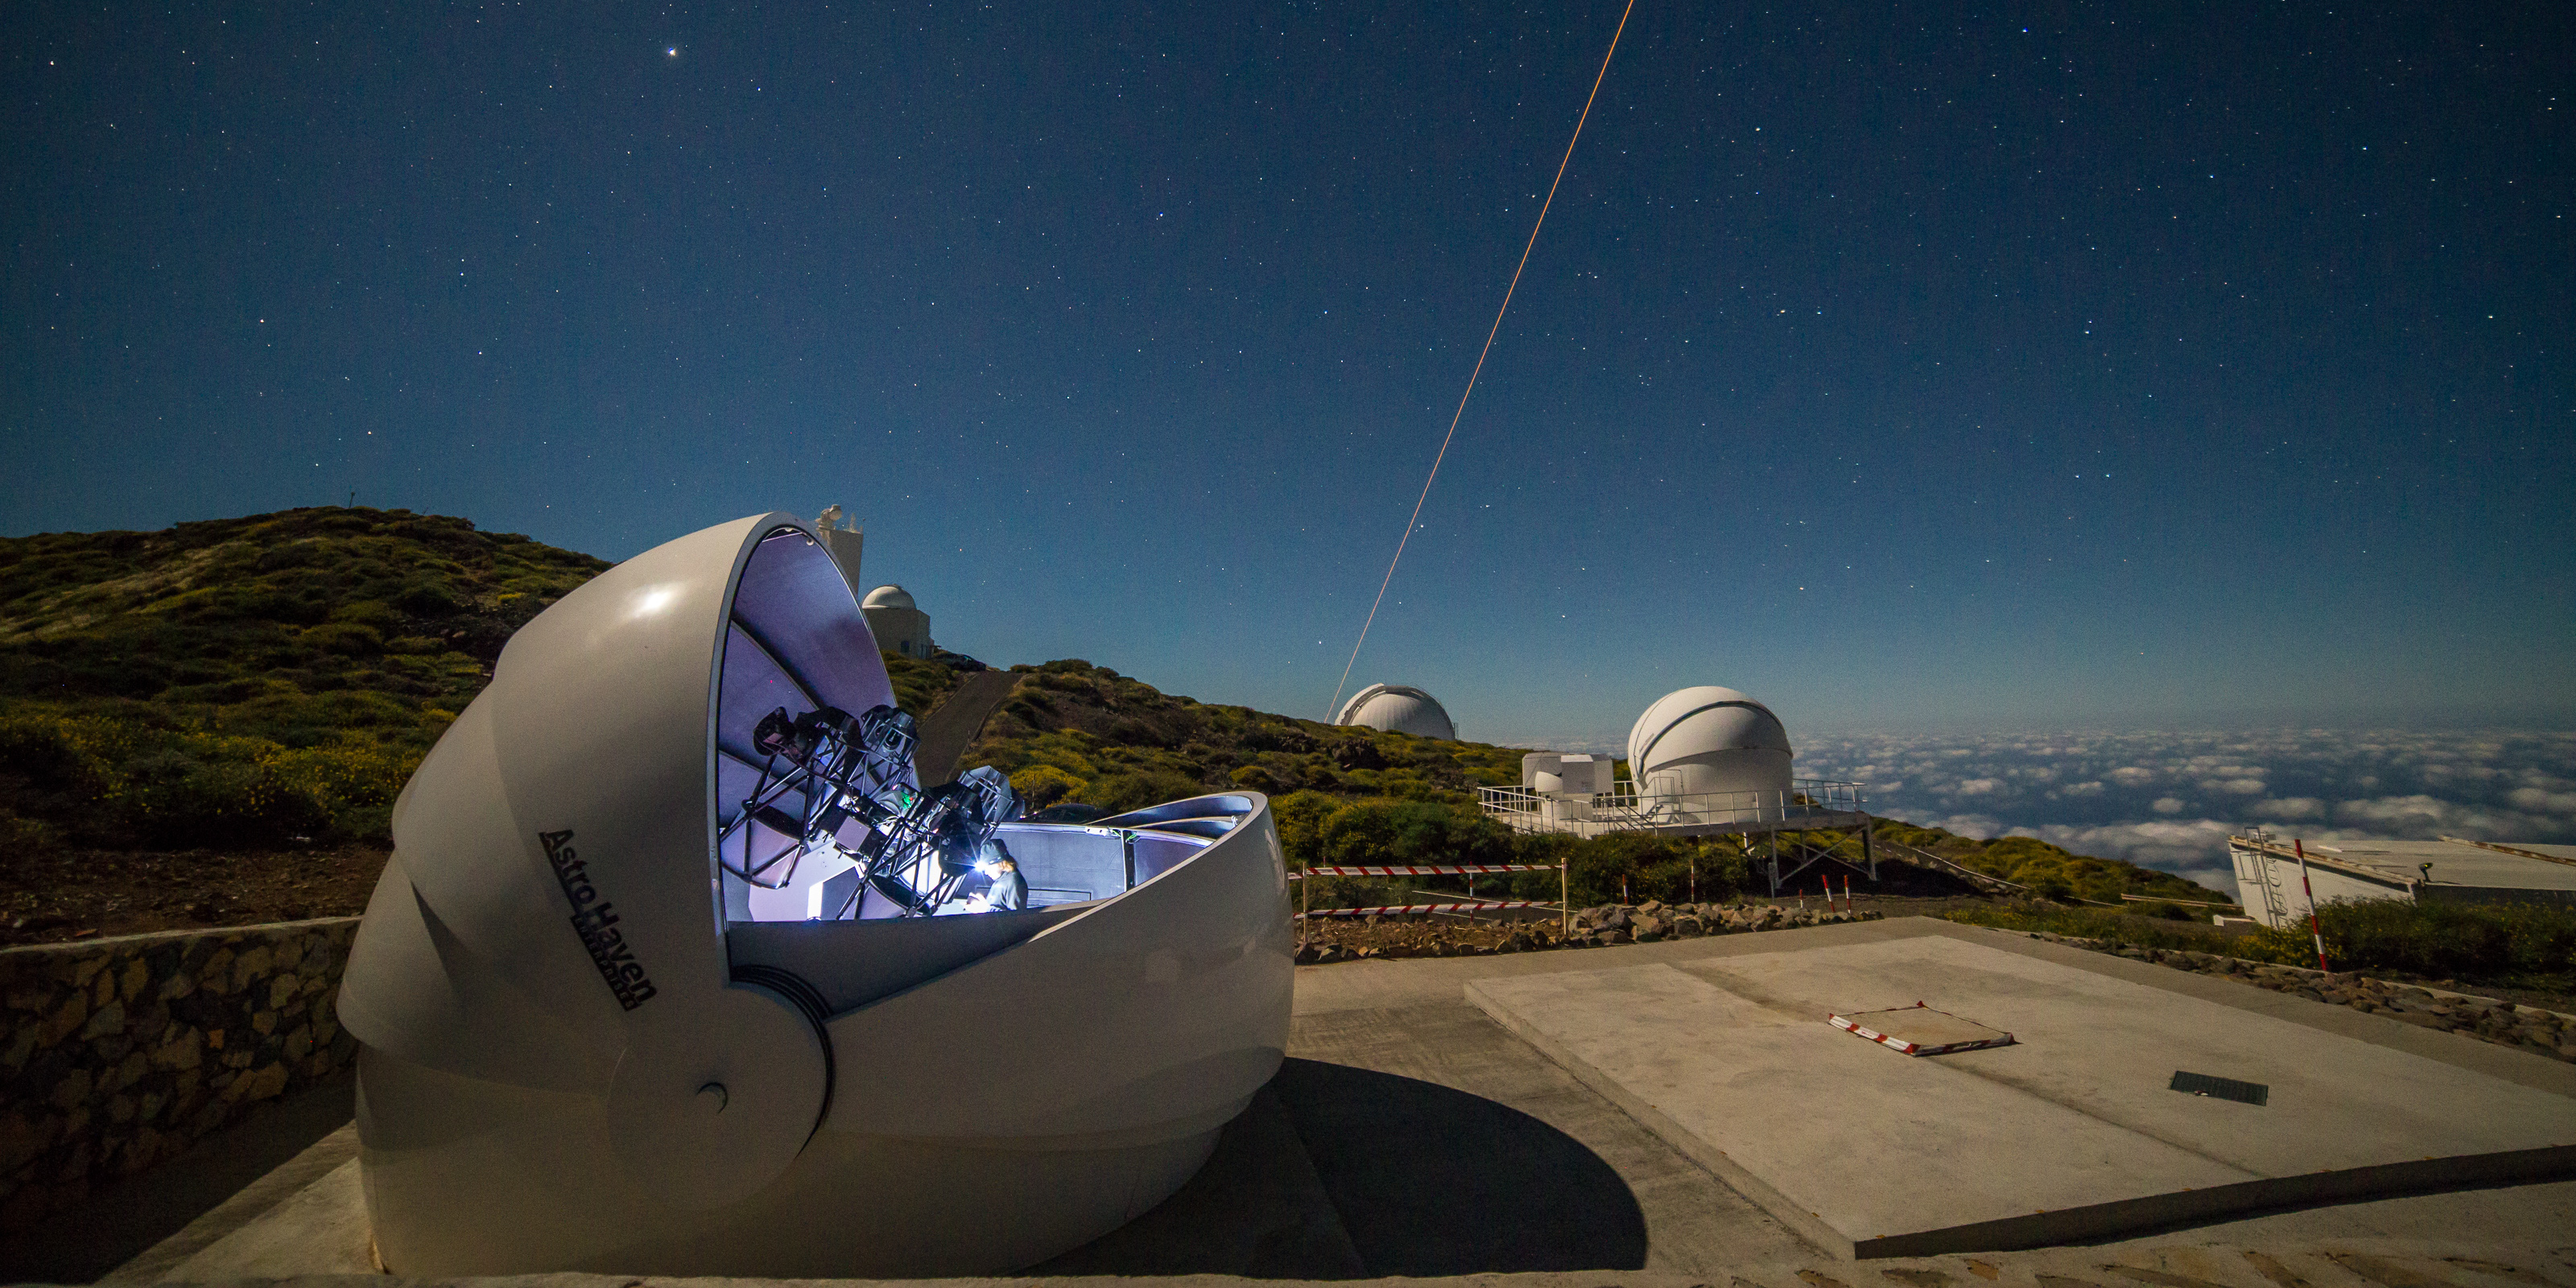
\includegraphics[width=\linewidth]{images/inauguration_photo.jpg}
    \end{center}
    \caption[Working in the GOTO dome prior to the inauguration in June 2017]{
        Working in the GOTO dome prior to the inauguration in June 2017.
        Photo taken looking west towards W1m and the WHT (with the orange CANARY laser visible). The second dome was installed on empty platform to the right later in the year.
    }\label{fig:inauguration}
\end{figure}

Ultimately, the mount and first four unit telescopes were shipped to La Palma in late May 2017, and GOTO officially saw first light on the 10th of June 2017. I went out to the site a few weeks later, in order to install the G-TeCS software (an image of the site at the time is shown in \aref{fig:inauguration}). By the time of the inauguration ceremony on the 3rd of July the hardware control system was in place and working well, and I was able to demonstrate the telescope that evening to the assembled dignitaries.

I returned to the site less than two weeks later with Stu Littlefair, in order to do further work on the control software. We commissioned the pilot and developed the observing routines described in \aref{sec:software_commissioning}, and oversaw the telescope's first fully-autonomous night on the 27th of July.

Unfortunately, in the months after the inauguration problems began to surface with the hardware. The first problem was the failure of the declination motor encoder shortly after the inauguration (prior to my second visit). We were able to operate GOTO in a limited RA survey mode (described in \aref{sec:challenges}), however this greatly limited the capability of the telescope. There were also other problems with the mounting brackets that hold the unit telescopes to the boom arm becoming loose, as well as the boom arms being short enough that the unit telescopes could hit the mount pier. These issues meant that for the first few months of commissioning someone always needed to be present in the dome to stop the mount moving if it was in danger of damaging itself. Once the second LIGO observing run (O2) finished at the end of August there was less of a reason to be observing in this limited mode, so GOTO was shut down during the autumn of 2017 until hardware upgrades could be installed at the start of November.

At the same time, problems with the optical performance of the unit telescopes had become apparent, which were blamed on the mirror quality and issues with collimation. A program of sending each set of mirrors back to the manufacturer one at a time was decided on, allowing GOTO to continue operating with the remaining three unit telescopes. The worst performing telescope, UT3, had its mirrors taken out and returned in August 2017. Once the telescope was reactivated in November, the remaining three unit telescopes were aligned to form a single 3$\times$1 footprint, shown in \aref{fig:3ut_footprint}. Counterweights were placed in the empty UT3 tube to allow the mount to maintain balance.

GOTO operated in this mode for over a year. The gap between LIGO runs gave time to fully test the control software, as well as develop the GOTOphoto image pipeline (see \aref{sec:gotophoto}). The first set of mirrors were returned to the site in June 2018 and were placed into UT4, which was the second-worst performing telescope. The old UT4 mirrors were then sent back to the manufacturer, and GOTO continued to operate with three unit telescopes until February 2019. At this point, based on the imminent start of the third LIGO-Virgo observing run (O3), it was decided to leave the UT1 and UT2 mirrors in place, and operate from then on in the 4-UT configuration. The resulting 2$\times$2 footprint is shown \aref{fig:4ut_footprint}. Note the unit telescopes are arranged with overlapping fields of view, to counteract for the poor image quality off-axis. With future optical improvements this overlap could be reduced, increasing the overall field of view.

\begin{figure}[p]
    \begin{center}
        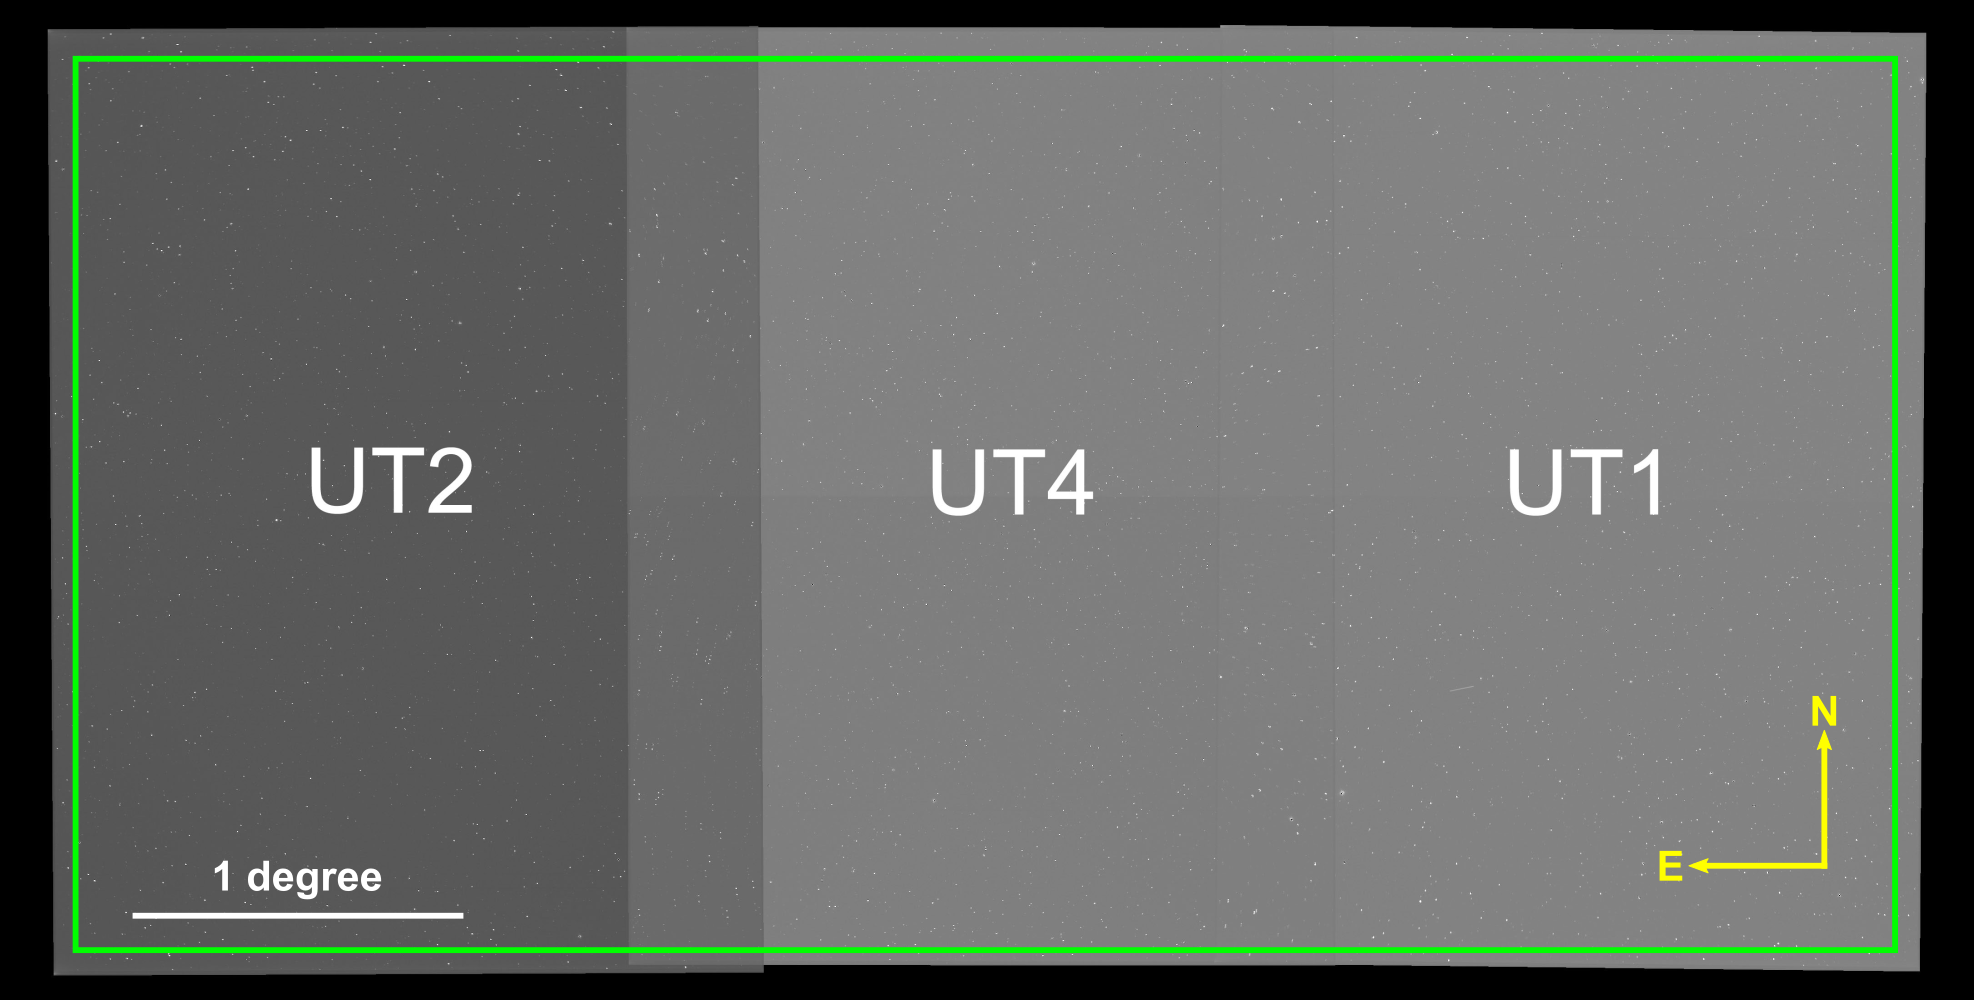
\includegraphics[width=0.7\linewidth]{images/footprint_1_box.png}
    \end{center}
    \caption[The previous 3-UT GOTO footprint]{
        The 3-UT GOTO footprint, used from August 2017 to February 2019.
        The initial \SI{5.5}{\degree} $\times$ \SI{2.6}{\degree} tile area used by GOTO-tile (see \aref{chap:tiling}) is shown in \textcolorbf{Green}{green}. Note that a reasonable amount of space is left around the edge of the tile.
    }\label{fig:3ut_footprint}
\end{figure}

\begin{figure}[p]
    \begin{center}
        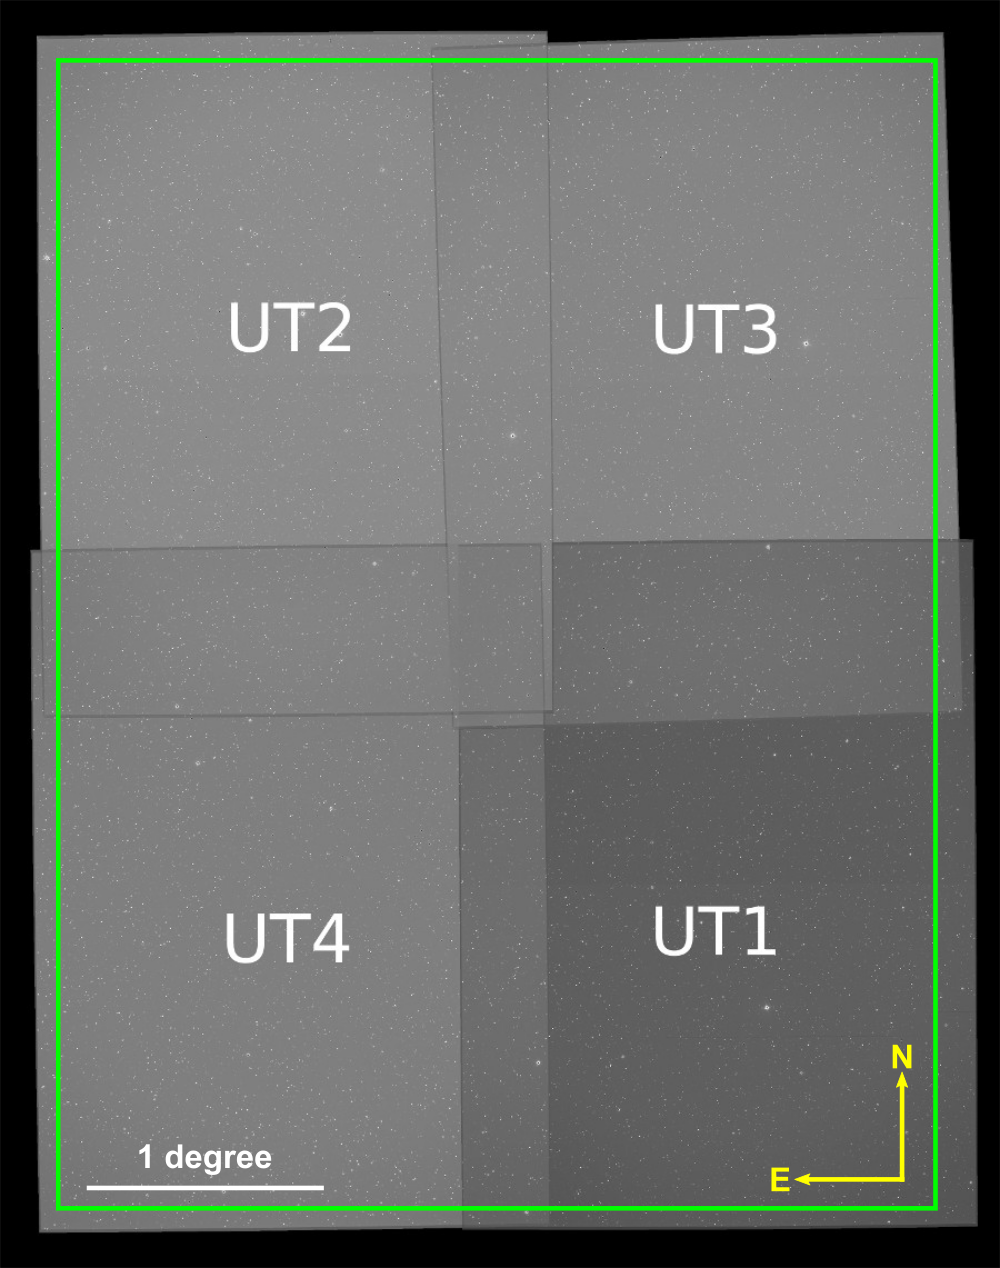
\includegraphics[width=0.55\linewidth]{images/footprint_2_box.png}
    \end{center}
    \caption[The current 4-UT GOTO footprint]{
        The current 4-UT GOTO footprint, in use from February 2019 onwards.
        The revised \SI{3.7}{\degree} $\times$ \SI{4.9}{\degree} tile area is shown in \textcolorbf{Green}{green}. The future four unit telescopes are expected to be arranged in two more columns on the left and right as shown in \aref{fig:fov}, creating an approximately \SI{7.8}{\degree}--wide footprint.
    }\label{fig:4ut_footprint}
\end{figure}

\newpage

Another problem found during commissioning was excessive scattered light entering the system, in particular light from the Moon entering the corrector lens (see the optical design in \aref{fig:ota}). This was solved by adding covers around the telescope tubes, which prevented light from entering the corrector but made the system more susceptible to wind-shake (the reason that the tubes were open in the first place). Ultimately the covers were found to provide enough benefits, including protecting the mirrors from dust, that it has been decided that future unit telescopes will have closed tubes.

\begin{figure}[t]
    \begin{center}
        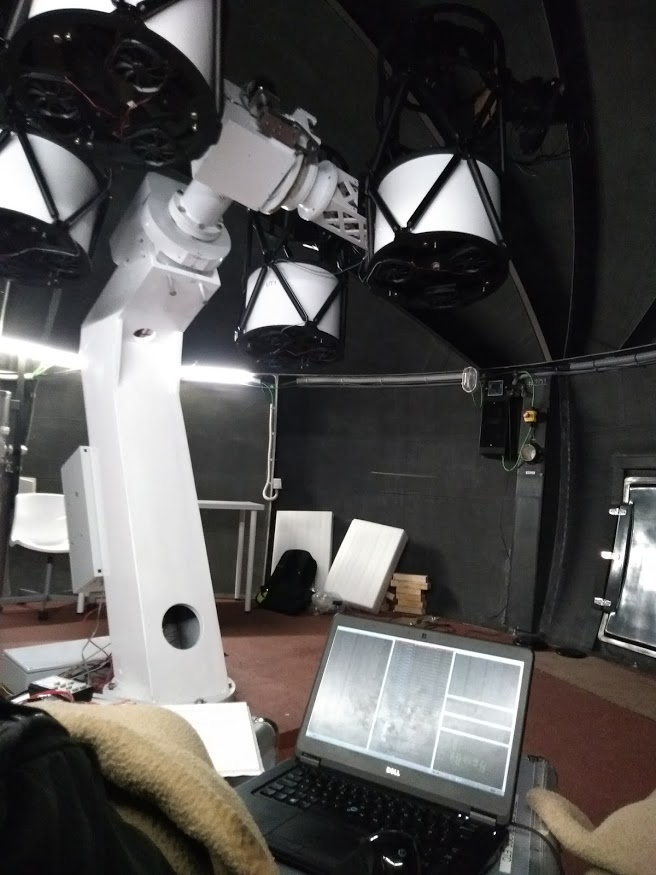
\includegraphics[width=0.4\linewidth]{images/commissioning_photo.jpg}
        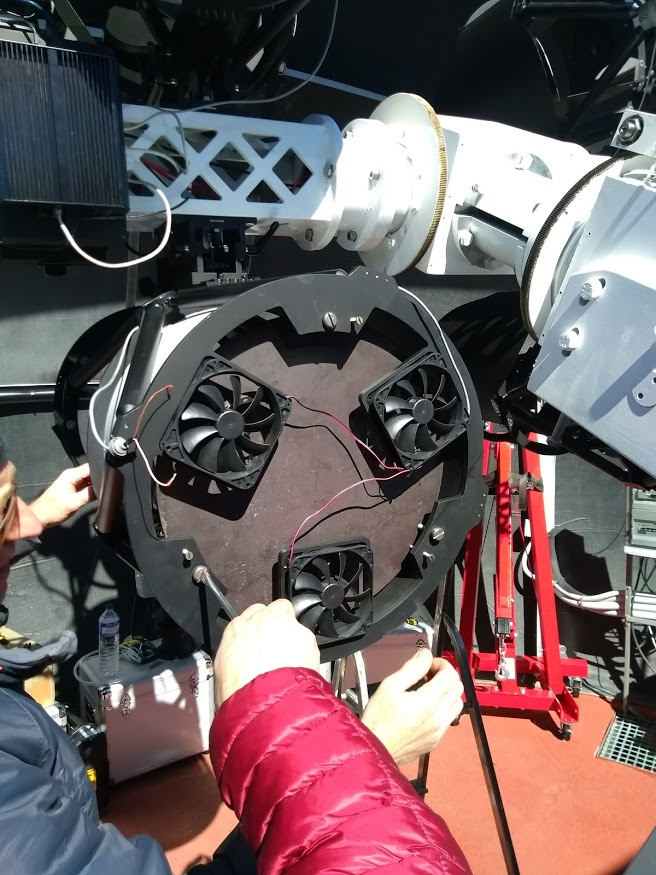
\includegraphics[width=0.4\linewidth]{images/commissioning_photo3.jpg}
    \end{center}
    \caption[Photos from GOTO commissioning]{
        Photos from GOTO commissioning: monitoring the telescope from inside the dome in November 2017 on the left, and fitting the mirror counterweights in UT3 in January 2018 on the right.
    }\label{fig:commissioning}
\end{figure}

The second commissioning period ran from the telescope being reactivated in November 2017 through to May 2018. During this time the telescope was typically running robotically each night, however there was always a member of the collaboration on site monitoring it in case of problems. Over that period the monitor moved from physically sitting in the dome (shown in \aref{fig:commissioning}), to sitting in the relative comfort of the neighbouring SuperWASP server room, until finally in the last few months being able to monitor from the observatory residencia or one of the other large telescopes on site.

I visited La Palma twice during this period, with the first trip in November 2017 covering the first week of the monitoring period immediately following the telescope being reactivated. Other volunteers monitored the system on-site until Christmas, then commissioning halted over the holiday period before I returned to the site in January for a three week visit. Kendall Ackley from Monash was also on site during the first week, and the first and third weeks overlapped with a team from Sheffield including Vik Dhillon and Stu Littlefair. During this period we replaced the counterweights (also shown in \aref{fig:commissioning}), rebalanced the mount and realigned the unit telescopes, and I continued the software work with a major update to the observation database. During the second week I monitored the telescope alone from SuperWASP, and continued developing the pilot so it was able to run automatically with no human supervision. In the third week I was due to remain on site and continue to monitor the telescope, however a severe snowstorm stopped all observing.

Due to the cold weather and ice build up GOTO was unable to open throughout all of February 2018. It was during this period that issues arose from the weight of the ice on the dome shutters, described in \aref{sec:challenges}. On-site monitoring resumed in the spring, once the snow had melted, and monitors continued to be on site for several more months, in between hardware upgrade trips lead by the Warwick team. Eventually in May the software was deemed robust enough to allow GOTO to run unsupervised. The pilot output is still regularly monitored remotely, especially from Australia by the Monash team, who have the benefit of a more convenient timezone.

By the time the 4-UT system was recommissioned, in February 2019, the G-TeCS pilot and hardware control systems had been fully tested and were operating reliably. By then my focus had shifted to the alert follow-up systems detailed in \aref{chap:alerts}, in advance of the start of O3 in April 2019. Since then GOTO has been reliably running and responding to gravitational-wave alerts, as detailed in \aref{sec:conclusion}.

\end{colsection}

% ~~~~~~~~~~~~~~~~~~~~

\subsection{Additional dome systems}
\label{sec:arduino}
\begin{colsection}

GOTO uses a clamshell dome manufactured by Astrohaven, the same company that made the pt5m dome \citep{pt5m}. Based on experience with p5tm, there were several hardware systems which we decided to add to the GOTO dome. In fact, the entire pt5m dome control unit was replaced by a custom one designed and manufactured in Durham, but we wanted to avoid taking such a drastic step. Several limitations of the stock Astrohaven dome are outlined below.
%
\begin{itemize}
    \item First, there was no easily-accessible emergency stop button to cut power to the dome in an emergency (e.g.\ something gets caught in the motors). This is a serious concern for pt5m, as when the dome is open the shutters completely cover the access hatch, making it dangerous for anyone to be passing through the hatch when the dome is moving. Therefore, one of the additions to pt5m was an emergency stop button within arms reach of the hatch entrance. As the GOTO dome is taller the hatch is mostly uncovered when the dome is open, but installing an emergency stop button was still a priority for safety reasons.
    \item The dome does not come with a siren to sound when it opens or closes. This is an important safety feature when operating a robotic observatory, as the dome will be operated entirely through software and it is important to warn anyone on site several seconds before it is about to move. When members of the GOTO team are on-site the robotic systems can be disabled entirely by going into engineering mode (see \aref{sec:mode}), however it is still important to make sure that there is no chance of the dome moving without prior warning. In addition, the GOTO site on La Palma is publicly accessible, and it is not unknown for tourists or hikers, or other astronomers, to be around the dome when it is unsupervised.
    \item By default, the dome \acro{plc} only provides limited information about the status of the dome shutters. As described in \aref{sec:dome}, the PLC only returns a single status byte in response to a query. This is not enough to distinguish whether the dome is fully or only partially open, and if one side is moving the status of the other side is unknown. Adding our own sensors would allow the complete status of the dome to be determined. The dome comes with two in-built magnetic sensors on each side, which should detect when the shutters are either fully closed or fully open. However these have been known to be unreliable and tricky to align. In some cases the switches failed to trigger when the shutter reached its open limit, leading to the dome continuing to drive the belts and the shutter embedding itself into the ground. Therefore having secondary, independent sensors was a priority to ensure this did not happen.
    \item The dome does not include a sensor on the hatch door to detect if it is open, and there is no way to close the hatch remotely in case of bad weather. As GOTO will be operating without anyone on site, the hatch should normally remain closed at all times, and by adding a sensor to the hatch this could be confirmed and an alert issued if the hatch is detected as open (see \aref{sec:conditions_flags}).
    \item One final proposed addition was a quick-close button, which acts as a simple and direct way to communicate with the dome daemon. The motivation is a practical one: in the case that the weather turns bad and the telescope is exposed, assuming the automatic monitoring systems fail and we can not connect to close it remotely, it is a lot easier and quicker to direct someone on site to access the dome and press the prominent ``close'' button than direct them to log on to the in-dome computer, open a terminal and type \code{dome~close}. This was also true during the commissioning phase, when the software was still being tested and someone has to be on-site all night. One requirement was that this button could not be easily confused with the emergency stop button (i.e.\ it should not be coloured red), as instead of stopping the dome this button will prompt it to move.
\end{itemize}

\begin{figure}[t]
    \begin{center}
        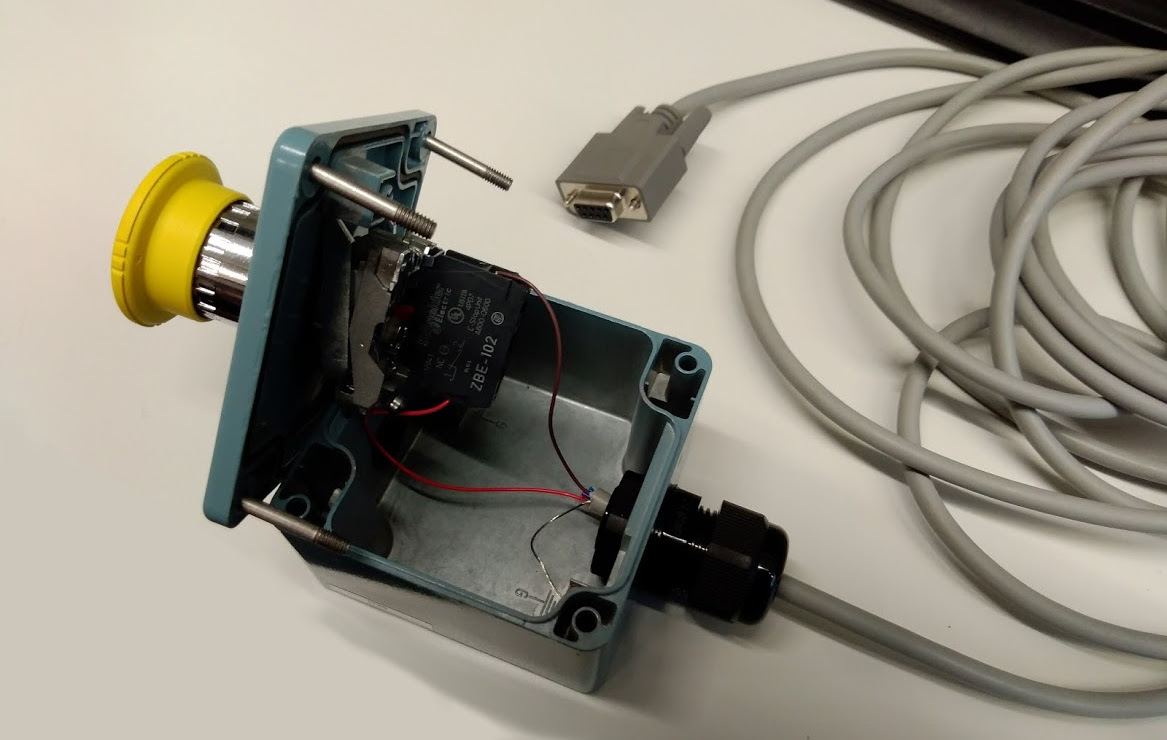
\includegraphics[width=0.9\linewidth]{images/button_photo.jpg}
    \end{center}
    \caption[Building the quick-close button]{
        Building the quick-close button in the lab. The transmit (\textcolorbf{Brown}{brown}) and receive (\textcolorbf{Red}{red}) wires from the serial cable are attached to the button NC pins.
    }\label{fig:quickclose_button}
\end{figure}

Creating a quick-close button involved attaching a ``normally closed'' (NC) push button in series between the transmit and receive wires of an RS 232 serial cable, as shown in \aref{fig:quickclose_button}. By doing this a simple feedback loop can be set up within the dome daemon, by sending a test signal out through the serial connection and listening for it to be returned to the same port. If after three tries the signal does not return then the button is assumed to have been pressed, and the dome daemon triggers a lockdown (see \aref{sec:dome}). By using a locking push button the loop will remain broken, and the dome closed, until the button is released. The bright yellow button was was labelled and attached to the wall of the dome near the computer rack (shown in \aref{fig:arduino_button_dome}).

Adding an emergency stop button to the dome was fairly simple. There was enough slack on the PLC power cable to install a prominent red button on the wall of the dome, as shown in \aref{fig:estop_plc}. When the button is pressed the power to the PLC and the dome motors is cut, which stops the dome moving.

\begin{figure}[p]
    \begin{center}
        \includegraphics[width=0.8\linewidth]{images/estop_photo.jpg}
    \end{center}
    \caption[The dome PLC and emergency stop button]{
        The dome \acro{plc} and emergency stop button. The green cable comes directly from the dome power supply at the top, passes through the button unit and into the PLC at the bottom.
    }\label{fig:estop_plc}
\end{figure}

\newpage

Adding a siren and additional sensors to the dome required an additional system to power, monitor and (for the siren) activate them. This was done using a small Arduino Uno microcontroller\footnote{\url{https://www.arduino.cc}} running a simple HTML server, which reports the status of the switches and can be queried in order to activate the siren. The circuit design for this system is shown in \aref{fig:arduino_circuit}. In order to power the siren from the Arduino a bipolar MOSFET (metal-oxide-semiconductor field-effect transistor)\acroadd{mosfet} was used to connect to one of the board input/output pins, with a large enough resistor to prevent the voltage from destroying the board. The Arduino and siren were mounted within a weatherproof case, with output connectors for the dome switches as well as for power and an ethernet connection. Photos of the box during construction are shown in \aref{fig:arduino_wip}, and its installation in the dome is shown in \aref{fig:arduino_installed} and \aref{fig:arduino_button_dome}.

\begin{figure}[t]
    \begin{center}
        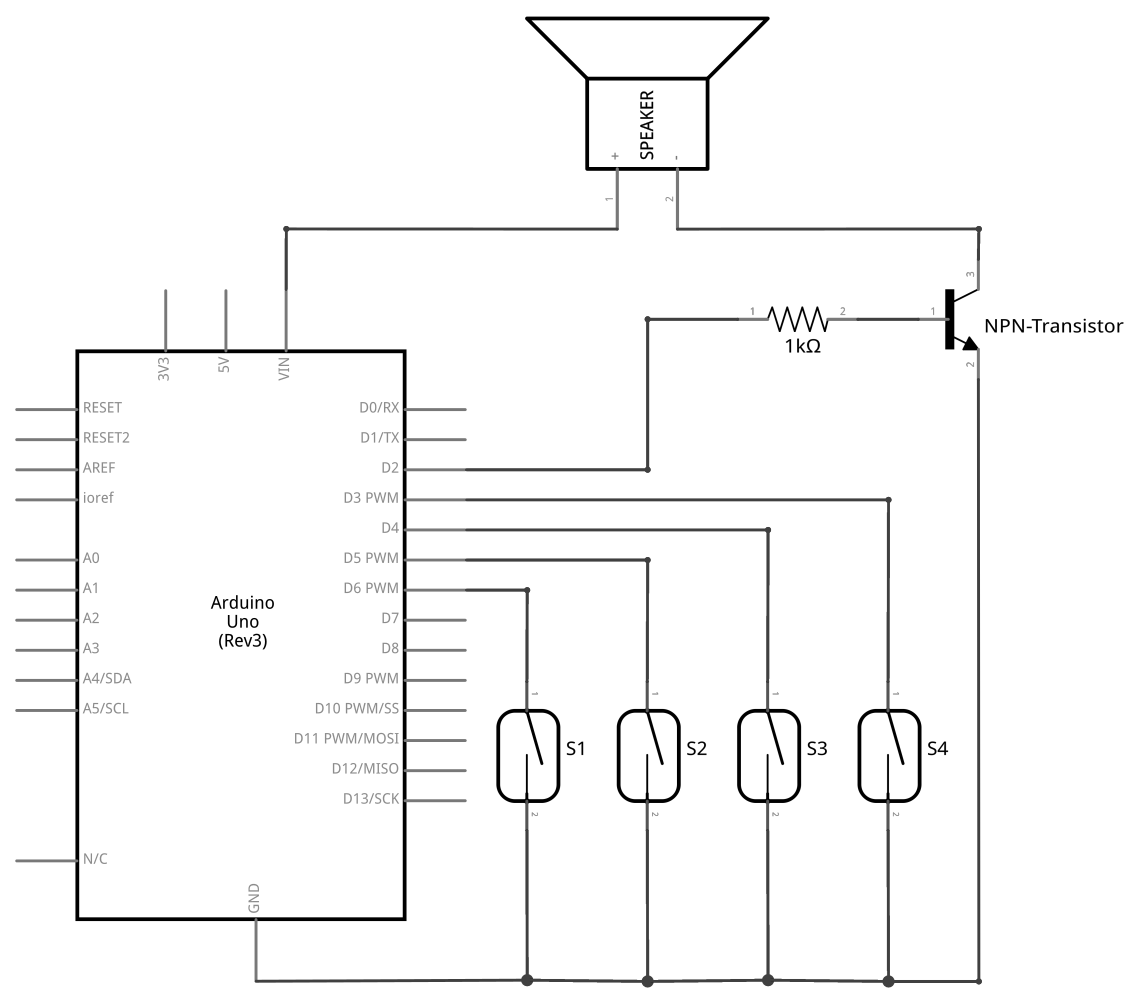
\includegraphics[width=0.75\linewidth]{images/arduino.png}
    \end{center}
    \caption[Circuit design for the Arduino box]{
        Circuit design for the Arduino box.
    }\label{fig:arduino_circuit}
\end{figure}

\newpage

\begin{figure}[p]
    \begin{center}
        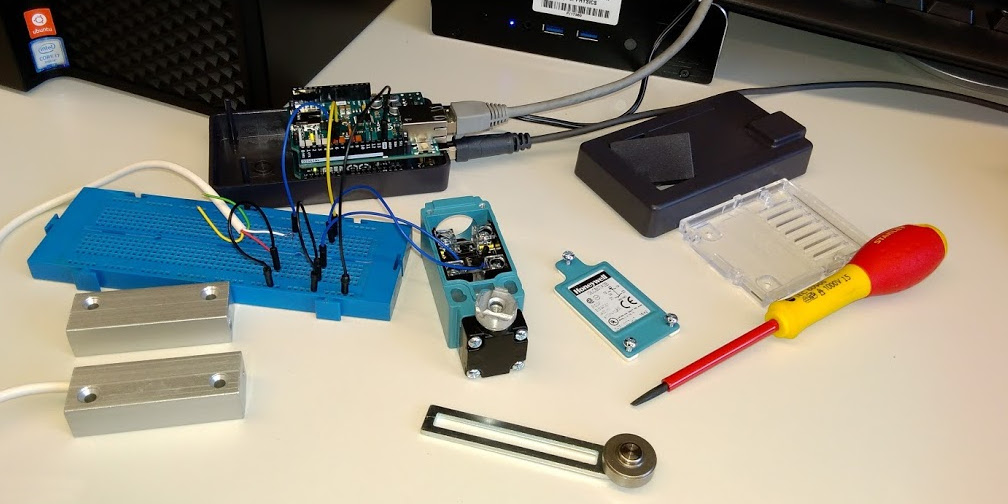
\includegraphics[width=\linewidth]{images/arduino_photo.jpg}
        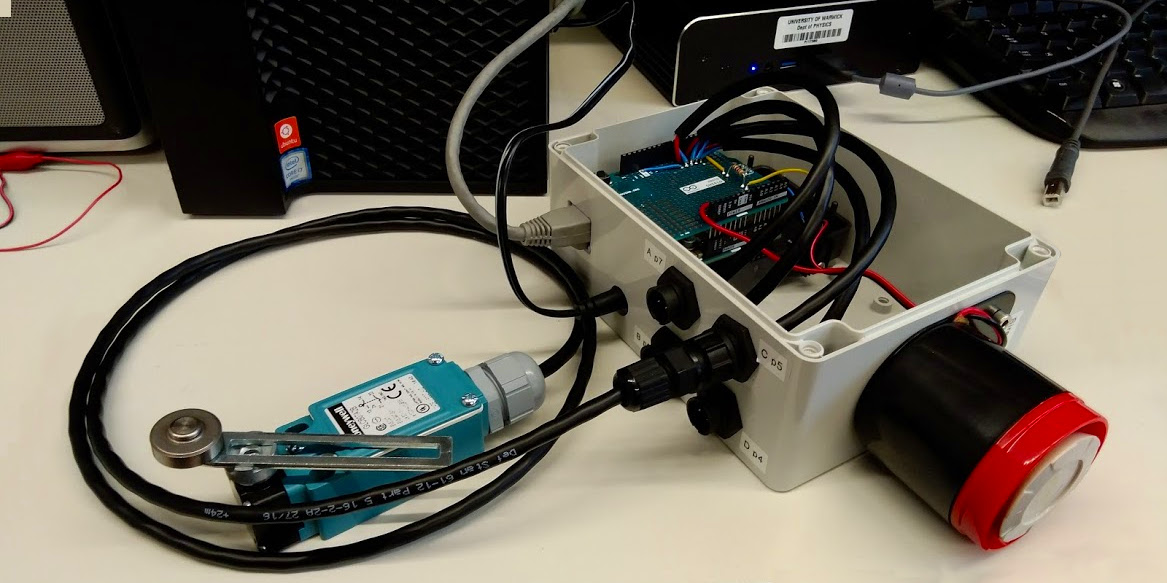
\includegraphics[width=\linewidth]{images/box_photo.jpg}
    \end{center}
    \caption[Building the dome Arduino box]{
        Building the dome Arduino box in the lab in Sheffield. The top image shows the circuit design being tested, with the Arduino (circuit board in the back) and two of the dome switches: a magnetic proximity switch (grey blocks on the left) and a Honeywell limit switch (cyan unit in the centre, with the cover and arm detached). The lower image shows the completed weatherproof box with the siren, power and ethernet cables and one of the Honeywell switches attached.
    }\label{fig:arduino_wip}
\end{figure}

\newpage

\begin{figure}[p]
    \begin{center}
        \includegraphics[width=0.75\linewidth]{images/box_installed_photo.jpg}
    \end{center}
    \caption[The Arduino box installed in the GOTO dome]{
        The Arduino box installed in the GOTO dome during my first trip to La Palma in March 2017. This photo was taken before the cover and cables were attached.
    }\label{fig:arduino_installed}
\end{figure}

\begin{figure}[p]
    \begin{center}
        \includegraphics[width=0.75\linewidth]{images/box_installed_photo2.jpg}
    \end{center}
    \caption[The Arduino box and quick-close button in the GOTO dome]{
        The Arduino box and yellow quick-close button in the GOTO dome, attached to the southern pillar under the dome drive. The cables run to the computer rack which is just off to the left of the photo.
    }\label{fig:arduino_button_dome}
\end{figure}

\clearpage

Four additional sensors were added to the dome, each connected to a port on the Arduino through the connectors on the bottom of the weatherproof box. Two Honeywell limit switches were attached to the rim of the dome wall, set to be triggered when the dome was fully open; additional magnetic proximity switches were added to the two inner-most shutters, which trigger when the dome is fully closed; and a magnetic proximity switch was added to the dome hatch. Each of these are shown in \aref{fig:dome_switches}.

\begin{figure}[p]
    \begin{center}
        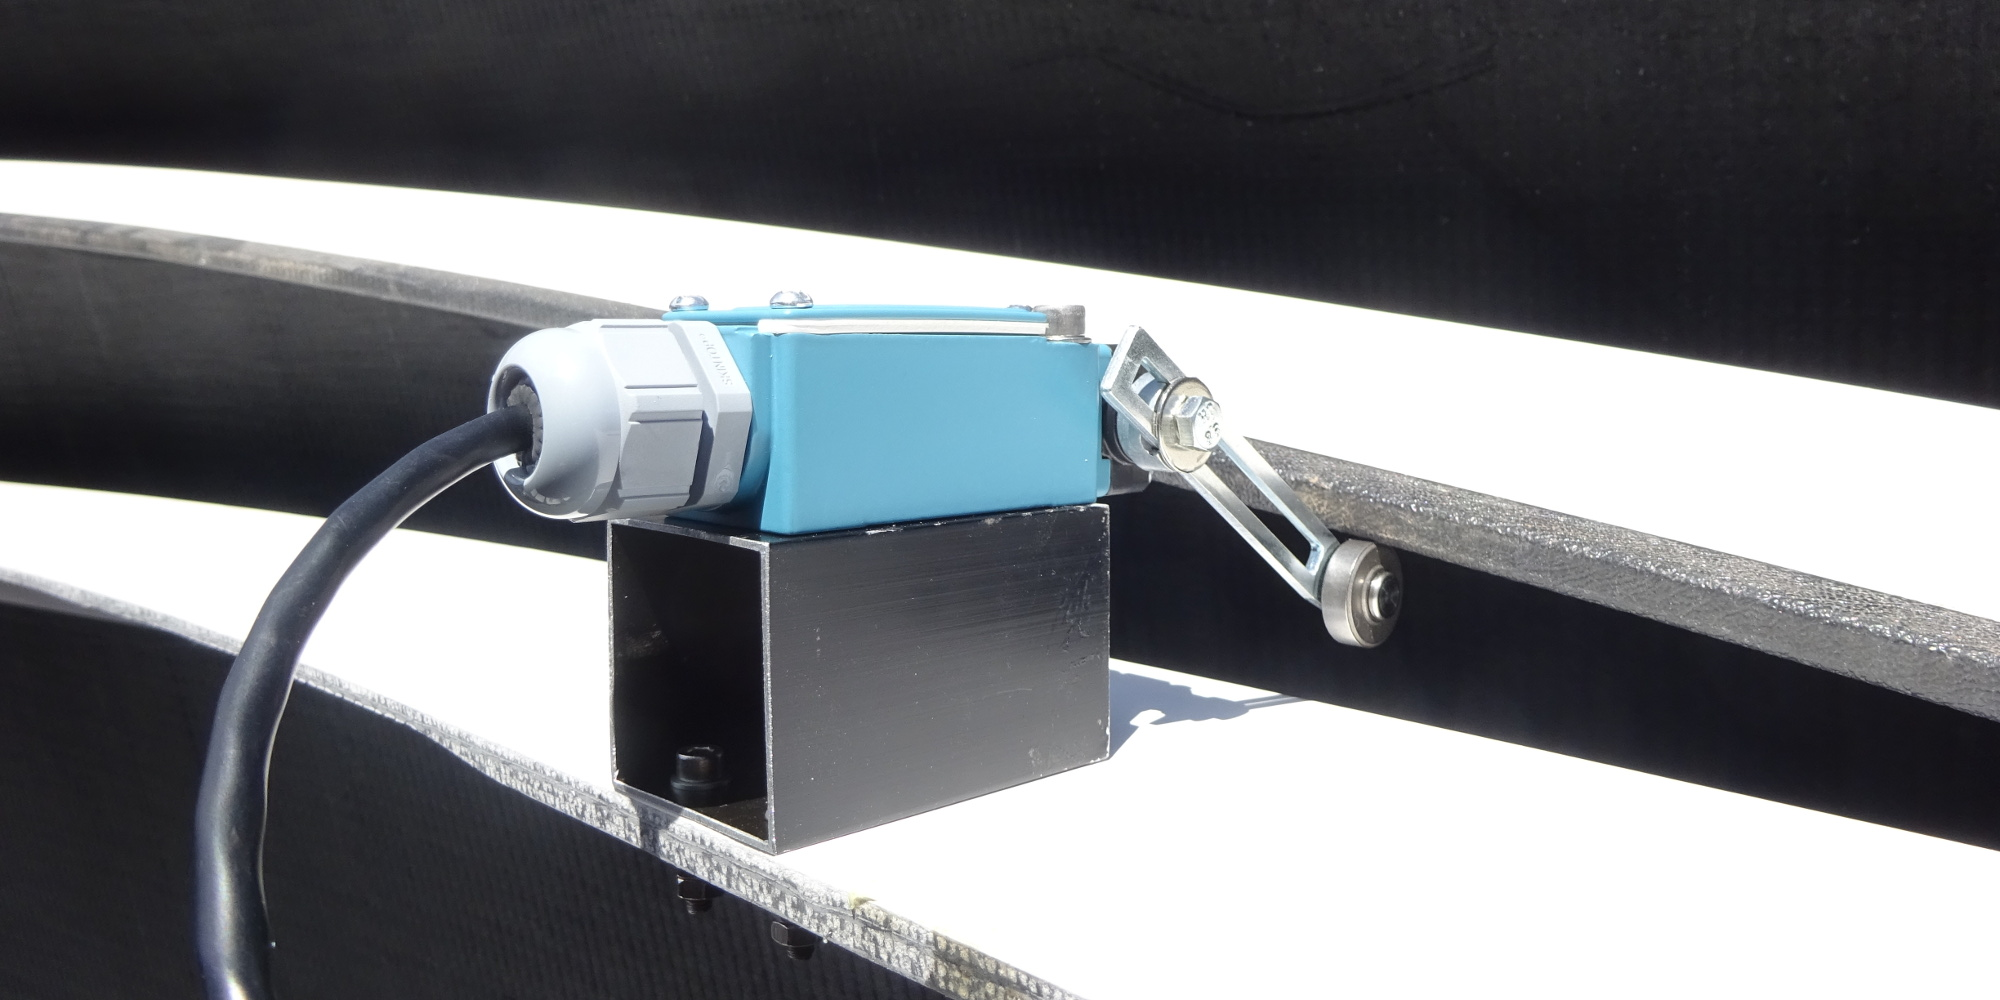
\includegraphics[width=0.8\linewidth]{images/dome_sensor_1.jpg}
        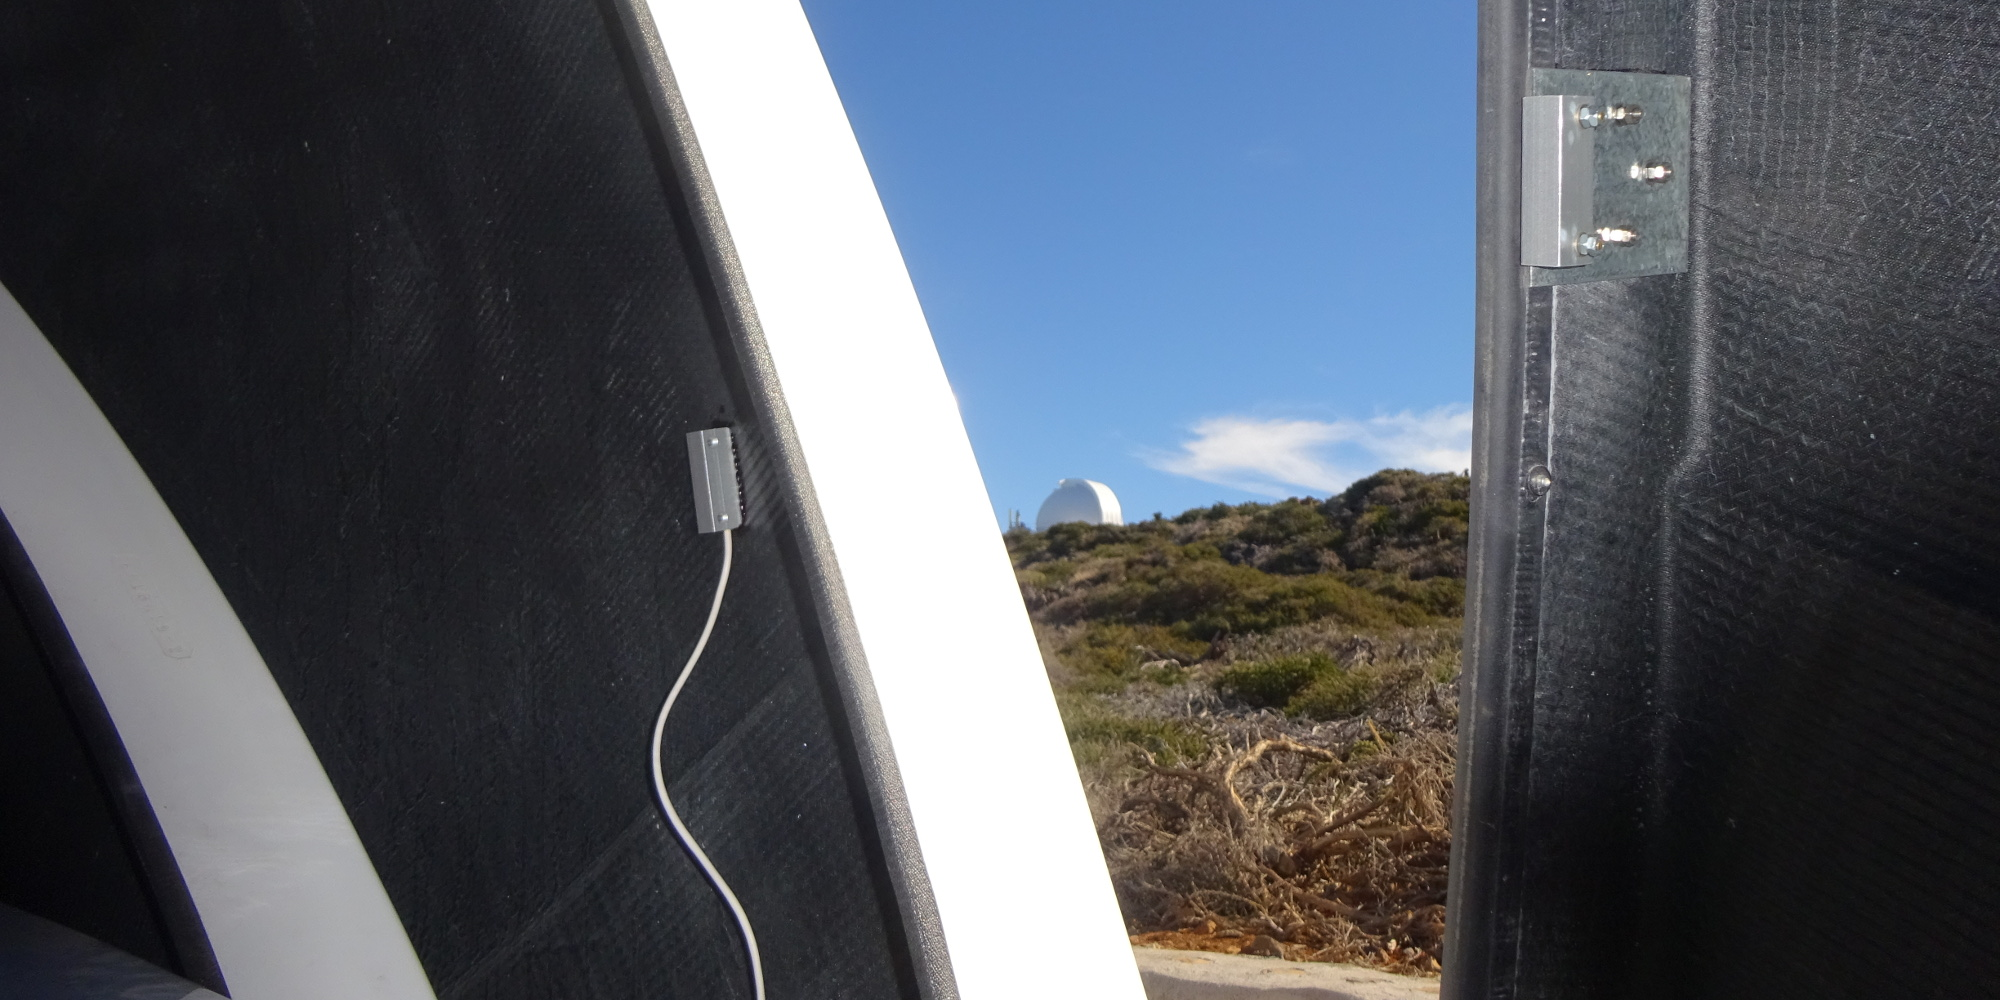
\includegraphics[width=0.8\linewidth]{images/dome_sensor_2.jpg}
        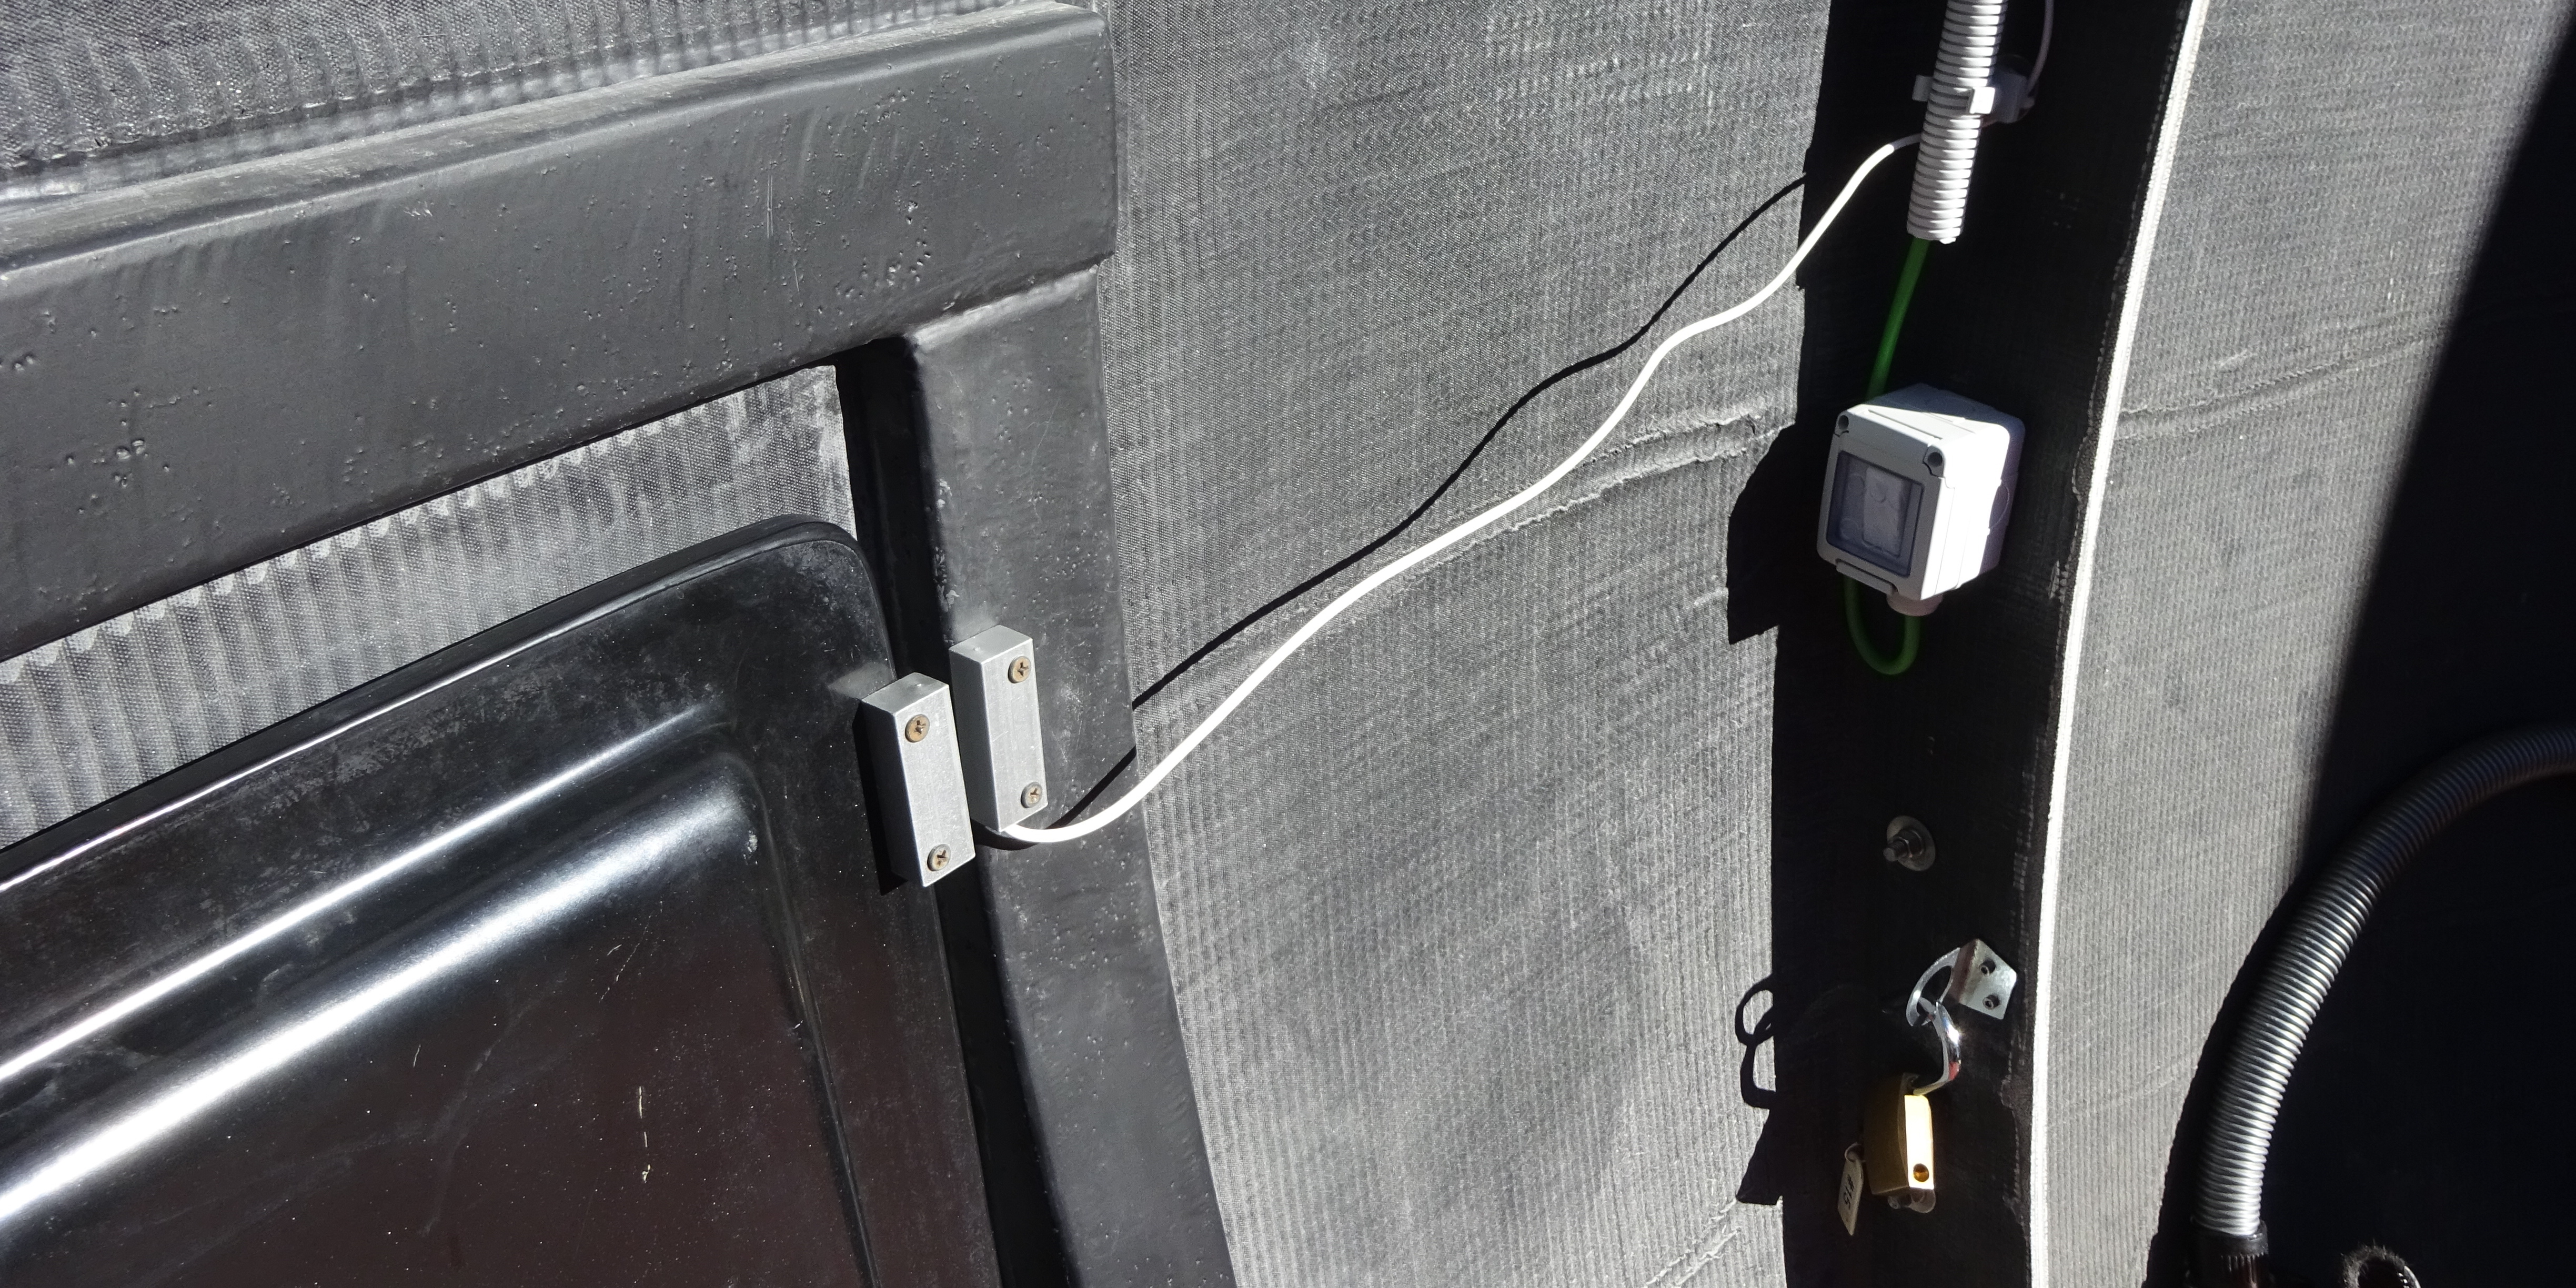
\includegraphics[width=0.8\linewidth]{images/dome_sensor_3.jpg}
    \end{center}
    \caption[Additional sensors added to the dome]{
        Additional sensors added to the dome. The top photo shows one of the two Honeywell limit switches added to the rim of the dome wall to detect when the dome is fully open, the middle photo shows magnetic switch added to the inner-most shutters to detect when the dome is fully closed, and the bottom photo shows the magnetic switch added to the dome hatch to detect when it is open.
    }\label{fig:dome_switches}
\end{figure}

Using a combination of these new switches and the PLC output it is possible for the dome daemon to build a complete picture of the status of the dome, as described in \aref{sec:dome}. Having a sensor on the hatch also allowed it to be added as a conditions flag, as described in \aref{sec:conditions_flags}, meaning the pilot will stop and report if the hatch is open when in robotic mode. As of yet, the hatch flag or in-dome buttons have not been needed in an emergency, however they are important as an insurance policy just in case. It is anticipated that the same work will need to be done in the second GOTO dome when it is commissioned. Comments have also been passed on to the dome manufacturer to suggest that they could include some of the features described in this section in their own stock hardware.

One further addition to the GOTO dome should be mentioned: the ``heartbeat'' monitor designed and installed by Paul Chote at Warwick. As described in \aref{sec:dome}, in the event that the dome daemon crashes, or the control NUC itself fails for whatever reason, the dome would be left vulnerable --- especially if it is already open. As a backup, Paul created his own Arduino system that connects to the dome PLC and sends it commands to close in the event that it does not receive a regular signal from the dome daemon. This system was installed into the GOTO dome in April 2018, along with the other Warwick domes on the site, and was one of the final stages required before GOTO could safely leave the commissioning phase and not require an on-site monitor. The two Arduino systems may be merged when the second GOTO dome is commissioned.

\end{colsection}

% ########################################

\section{Developing the software}
\label{sec:software_commissioning}

% ~~~~~~~~~~~~~~~~~~~~

\begin{colsection}

While the GOTO hardware was being commissioned the G-TeCS control software was also being developed. There were several important parts of the software that could not reasonably be developed without access to the actual telescope, for example the observing routines for taking flat fields and autofocusing.

This section focuses on the software side of commissioning, and does not include pure hardware issues such as with the mount drive, mirrors or UT brackets outlined in \aref{sec:timeline}. These were dealt with by the core GOTO hardware team at Warwick, and although I spent many hours on La Palma balancing the mount, adjusting mirror positions and aligning unit telescopes, it had limited impact on the control software development.

\end{colsection}

% ~~~~~~~~~~~~~~~~~~~~

\subsection{Taking flat fields}
\label{sec:flats}
\begin{colsection}

GOTO uses the twilight sky for taking flat fields. Some care has to be taken to design a reasonable flat-field routine, as taking sky flats is not simple for a wide-field instrument such as GOTO \citep{flats3, flats2}. As described in \aref{sec:night_marshal}, the night marshal runs the \code{take\_flats.py} observing script at twilight twice a day, once in the evening and again in the morning. In the evening the script begins after the dome is opened, when the Sun has set below \SI{0}{\degree} altitude, and in the morning the routine is run in reverse, starting after observations have finished and running until the Sun rises above \SI{0}{\degree}.

First, the telescope needs to slew to a chosen position. Based on the analysis of the twilight sky gradient in \citet{flats}, GOTO slews to the ``anti-sun'' position, which is at an azimuth of \SI{180}{\degree} opposite the position of the Sun and at an altitude of \SI{75}{\degree}. This should be the position where the sky gradient is minimised and therefore the field is flattest. In the pt5m version of the script, the telescope would slew to one of a predefined set of empty sky regions, however with GOTO's large field of view there are no large enough regions devoid of bright stars (to counter this, the mount moves slightly between images so that median stacking the frames will remove any stars).

Once the telescope is in position, glance exposures (see \aref{sec:cam}) are taken until the sky brightness has reached an appropriate level. In the evening, exposures start at $E_0=\SI{3}{\second}$ soon after sunset, and the first images will almost always be saturated. Images are taken until the mean count level has fallen below the target level of 25,000 counts per pixel. In the morning, exposures start at $E_0=\SI{40}{\second}$ while the sky is still dark, and exposures are taken until the mean count level is above the same target level.

Once the sky has reached the target level of brightness, exposures are taken at increasing exposure times in the evening, or decreasing in the morning. The exposure time sequence is determined using the method of \citet{flats3}, which defines the delay between exposures iteratively from $t_0=0$ using
%
\begin{equation}
    t_{i+1} = \frac{\ln{(a^{t_i+\Delta t} + a^{E_i} -1)}}{\ln{a}},
    \label{eq:sky}
\end{equation}
%
where $\Delta t$ is the time between exposures (including readout time and any offset slew time) and $a$ is a scaling factor which depends on the twilight duration $\tau$ in minutes as
%
\begin{equation}
    a = 10^{\pm 0.125/\tau}.
    \label{eq:sky2}
\end{equation}
%
The twilight duration can be calculated easily using Astropy, and $a$ is taken as less than 1 in the evening (the delay between exposures decreases) or greater than 1 in the morning (the delay increases). Note that $t$ is the time delay \emph{between} exposures, the actual exposure time of each exposure is given by
%
\begin{equation}
    E_{i+1} = t_{i+1} - (t_i + \Delta t).
    \label{eq:sky3}
\end{equation}

Using this method a sequence of exposure times is determined iteratively either until a target number of flat fields have been taken (by default 5 in each filter) or the exposure times pass a given limit (greater than \SI{60}{\second} in the evening, less than \SI{1}{\second} in the morning). Between each exposure the telescope is stepped 10~arcminutes in both RA and declination, enough to ensure that any objects in the field do not fall on the same CCD pixels. This means any stars in the field can be removed by median combining the individual flat field images.

Every time the script is run, flat fields are taken in each of the Baader \textit{LRGB} filters used by GOTO (see \aref{sec:filters}). In the evening flats start in the \textit{B} filter (as the sky progressively reddens as the Sun sets), progresses through \textit{G} and \textit{R}, and finishes on \textit{L} (as the \textit{L} filter has the widest bandpass). In the morning the sequence is reversed. Once the first set of flats is taken in the starting filter (\textit{B} in the evening, \textit{L} in the morning) a new starting exposure time ($E_0$) is calculated based on the relative difference in the filter bandpasses (see \aref{sec:filters}).

This method allows a reasonable set of flat fields to be taken in each filter most nights. The GOTOphoto pipeline (\aref{sec:gotophoto}) creates new master flat frames each month (the same is true of bias and dark frames); this means that taking new flats each night is important but not critical. If, for example, the Moon is too close to the anti-Sun point then flats can be skipped without causing any disruption. The routine also assumes a clear night and does not account for the presence of clouds in the field, however any poor-quality images are rejected by the pipeline when creating the master frames, and by taking new flats twice each night there should always be enough to create a valid master frame each month.

\end{colsection}

% ~~~~~~~~~~~~~~~~~~~~

\subsection{Focusing the telescopes}
\label{sec:autofocus}
\begin{colsection}

The GOTO unit telescopes are designed to keep a stable focus through the night, and use carbon-fibre trusses to minimise any changes due to temperature fluctuations. Based on images taken during commissioning this is generally true, and the pilot only has to refocus the telescope once at the start of each night. Once the flats routine has finished the night marshal within in the pilot runs the \code{autofocus.py} observing script (see \aref{sec:night_marshal}). To save time, all of the unit telescopes are focused at the same time, although completely independently.

The autofocus routine is based on the V-curve method of \citet{autofocus}, which measures the focus using the \acro{hfd}. The HFD is defined as the diameter of a circle centred on a star in which half of the total flux lies inside the circle and half is outside. As this parameter is based only on the total spread of the flux and not on the maximum peak it is not disrupted due to seeing effects. Importantly, the HFD should vary linearly with focus position, forming a V-shaped curve with a fixed gradient either side of the best focus (unlike the FWHM, which forms a U-shaped, non-linear curve). The gradient of this V-curve (shown in \aref{fig:autofocus}) is a function of the telescope hardware: changes in seeing move the curve up and down while changes in temperature will move the curve side-to-side, but the shape should remain the same. Therefore, if the V-curve has been defined for the given telescope and you can find which part of the curve you are on, you can use the known gradient and intercept to move directly to the minimum point, which will give the best focus.

\begin{figure}[t]
    \begin{center}
        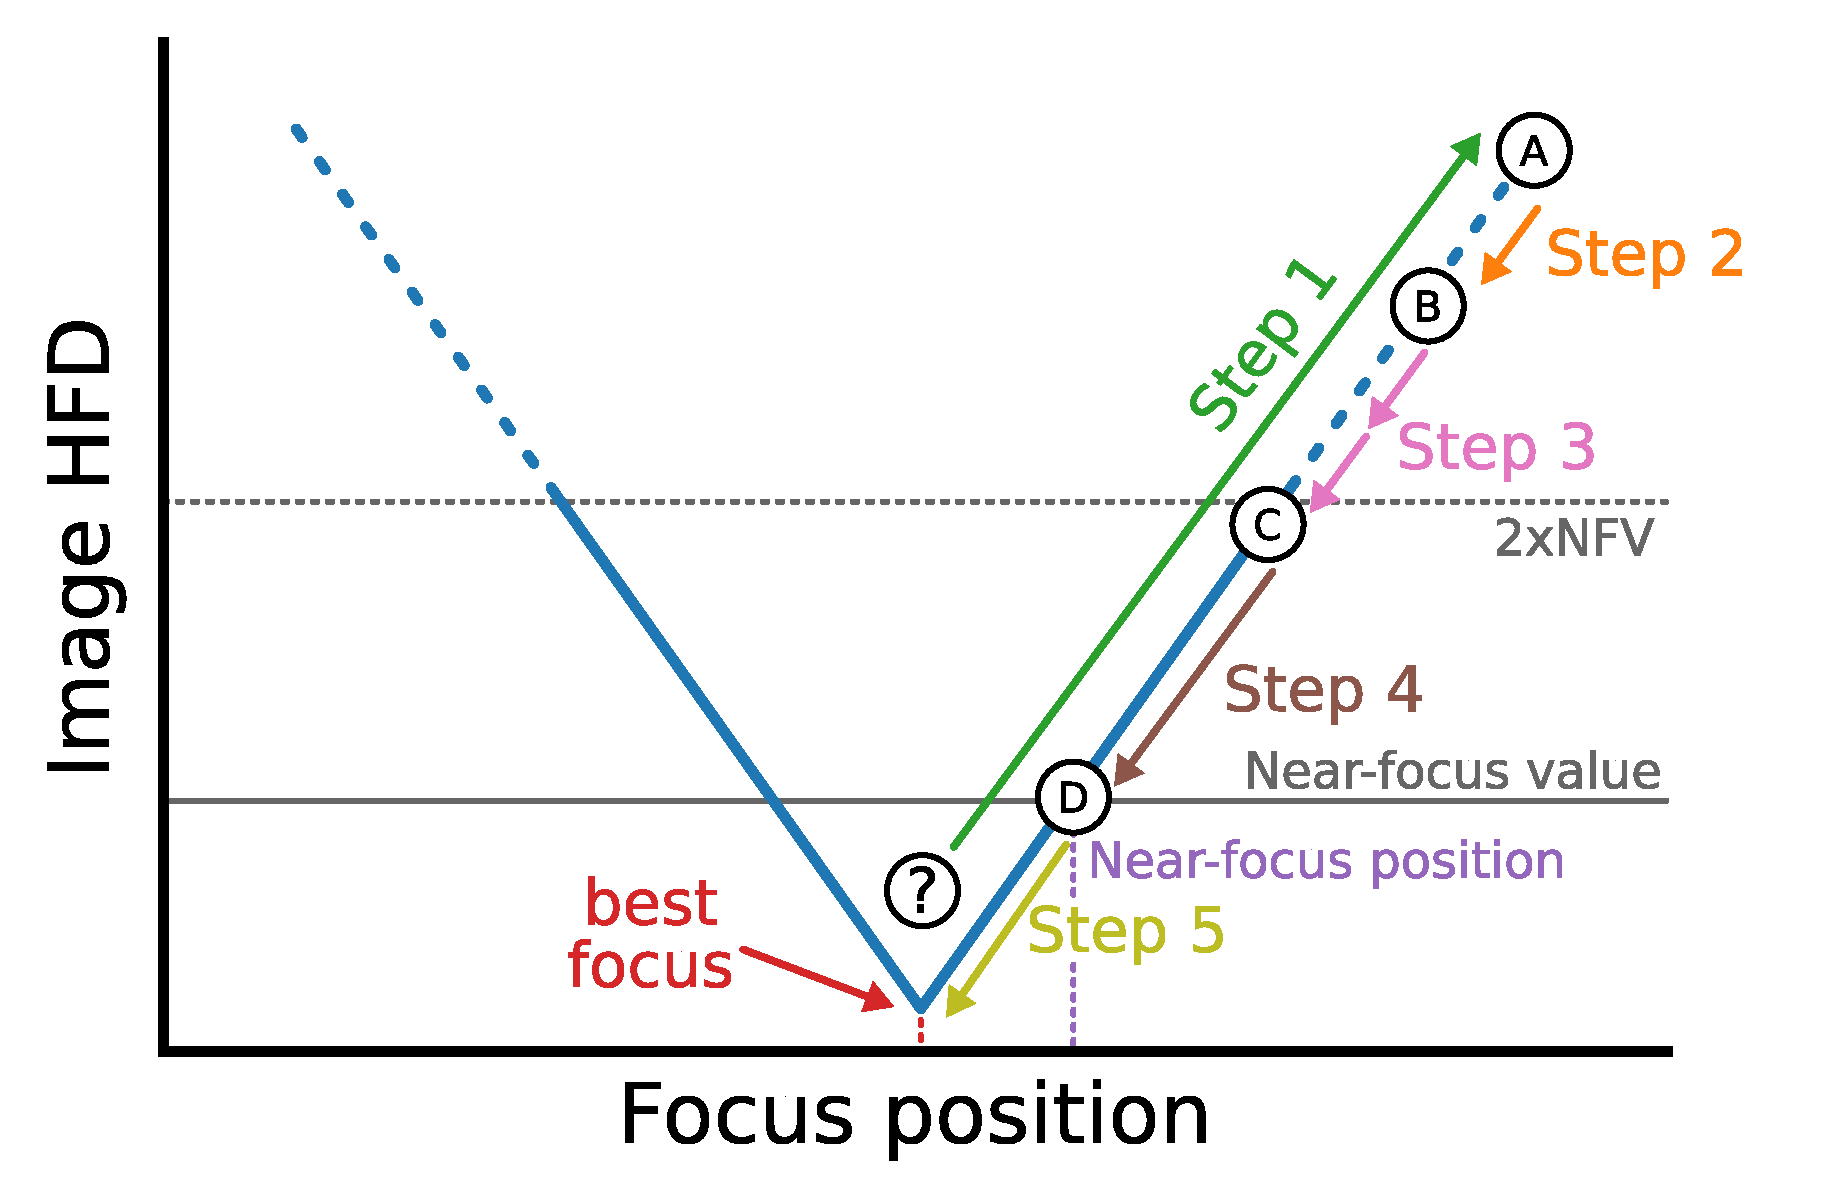
\includegraphics[width=0.8\linewidth]{images/autofocus.pdf}
    \end{center}
    \caption[Steps to find the best focus position using the HFD V-curve]{
        Steps to find the best focus position using the HFD V-curve.
    }\label{fig:autofocus}
\end{figure}

As GOTO is a wide-field instrument no particular focus star needs to be picked, and instead focusing takes place at zenith assuming that there are always enough stars to focus on within the field. Images are windowed to just a central 2000$\times$2000 pixel area, to avoid any distortions around the edge of the field. Sources are extracted and the half flux diameter measured using the SEP Python package (Source Extraction and Photometry, \pkg{sep}\footnote{\url{https://sep.readthedocs.io}}) which implements the Source Extractor algorithms in Python \citep{SE}. This is done for all objects in the frame with a signal of more than $5\sigma$ above the background sky, excluding any sources that do not match a Gaussian shape i.e.\ are not point sources. This typically results in several hundred sources in each unit telescope, and the mean of all of the points is taken as the representative HFD for that image.

At the start of the focus routine an initial image is taken and starting HFD values are measured. The starting focus position is also recorded at this point, so that if the script fails for any reason the initial focus can be restored. It is assumed that the initial value should be fairly close to the ideal focus position, but it is not known which side of the ideal position it is (i.e.\ if it is on the positive or negative gradient side of the V-curve). This starting point is shown by the \textbf{?} marker in \aref{fig:autofocus}.

The first step of the routine is to move the focuser by a large positive quantity, to point \textbf{A} in \aref{fig:autofocus}, and measure the HFD.\@ This is done to make sure that the image is completely de-focused, and we are on a known side of the best focus position. At this point the V-curve might not even be linear, but as long as the measured HFDs have increased compared to the starting value then we can proceed.

The second step is a small step back in the opposite direction, towards the best focus position (point \textbf{B}). The HFD is measured again, and it should now be smaller than when measured at point \textbf{A} but still larger than the starting value. If this is not true then the script returns an error, as it is not possible to determine if we are on the correct side of the V-curve.

The next stage is to continue taking small steps in the same (negative) direction, until the measured HFD is less than double the \emph{near-focus value} (NFV) \acroadd{nfv}. The NFV is chosen for each telescope to be a HFD value in pixels that is approximately equal to the expected best-focus value, based on previous measurements (for GOTO the NFV is 7 pixels). Once at this point (point \textbf{C}) we should be well within the linear portion of the V-curve. At this stage the exact HFD values are important, so three consecutive images are taken at this focus position and the smallest of the HFD values is taken as the first point on the V-curve. The HFD values between images will change due to external factors, such as seeing or windshake, but these will only ever make the HFD worse than the ``true'' value, never better. Therefore taking the minimum reduces the effect of these external factors on the measured HFD values.

Once the HFD value has been well measured at point \textbf{C} then the near-focus position (point \textbf{D}), the position that should produce a HFD equal to the near-focus value, can be found with
%
\begin{equation}
    F_\text{NF} = F + \frac{\text{NFV} - D(F)}{m_\text{R}}
    \label{eq:nearfocus}
\end{equation}
%
where $F$ is the current focus position, $D(F)$ is the current HFD and $m_\text{R}$ is the known negative gradient of the right-hand side of the V-curve --- this is just applying the equation of a straight line between two points.

Once the near-focus position has been found the focuser is moved to that position (point \textbf{D}) and the HFD is measured three times again. Now that we have a known $F_\text{NF}$ and $D(F_\text{NF})$ on the right-hand side of the V-curve the best focus position ($F_\text{BF}$) is given by the meeting point of the two lines shown in \aref{fig:autofocus}, which can be calculated using
%
\begin{equation}
    \begin{split}
                c_1 & = D(F_\text{NF}) - m_\text{R} F_\text{NF}, \\
                c_2 & = m_\text{L}(\frac{c_1}{m_\text{R}} - \delta), \\
        F_\text{BF} & = \frac{c_2 - c_1}{m_\text{R} - m_\text{L}},
    \end{split}
    \label{eq:bestfocus}
\end{equation}
%
where $m_\text{L}$ and $m_\text{R}$ are the gradients of the lines and $\delta$ is the difference between their intercepts. The focuser is then moved to the best focus position, the HFD values are recorded and the script is complete. This method has proven reliable to focus the GOTO telescopes on a nightly basis, although the optical aberrations produce badly-focused regions in the corners of the frames (described in \aref{sec:timeline}).

\aref{fig:focus_time} shows the focus values (half-flux diameter) measured from every image taken over a single night of observing. The HFD values vary between 3--5 pixels, and although there are some fluctuations there is no clear focus drift over the course of the night. \aref{fig:focus_temp} shows the same values plotted instead as a function of temperature, again no trends are visible. This is just a single sample from one night, and over a longer term there will be shifts in the best focus position. However, refocusing just once in the evening appears to produce a stable-enough position to last through the night.

It has been suggested that future GOTO unit telescopes might use an enclosed, prime-focus tube instead of the current Newtonian design with carbon fibre trusses (see \aref{sec:optics}). Solid metal tubes are much more sensitive to temperature variations and therefore need to continually be refocused during the night. To account for this a refocus step could be added into the exposure queue daemon (see \aref{sec:exq}) at the same stage that the filters are changed.

\begin{figure}[p]
    \begin{center}
        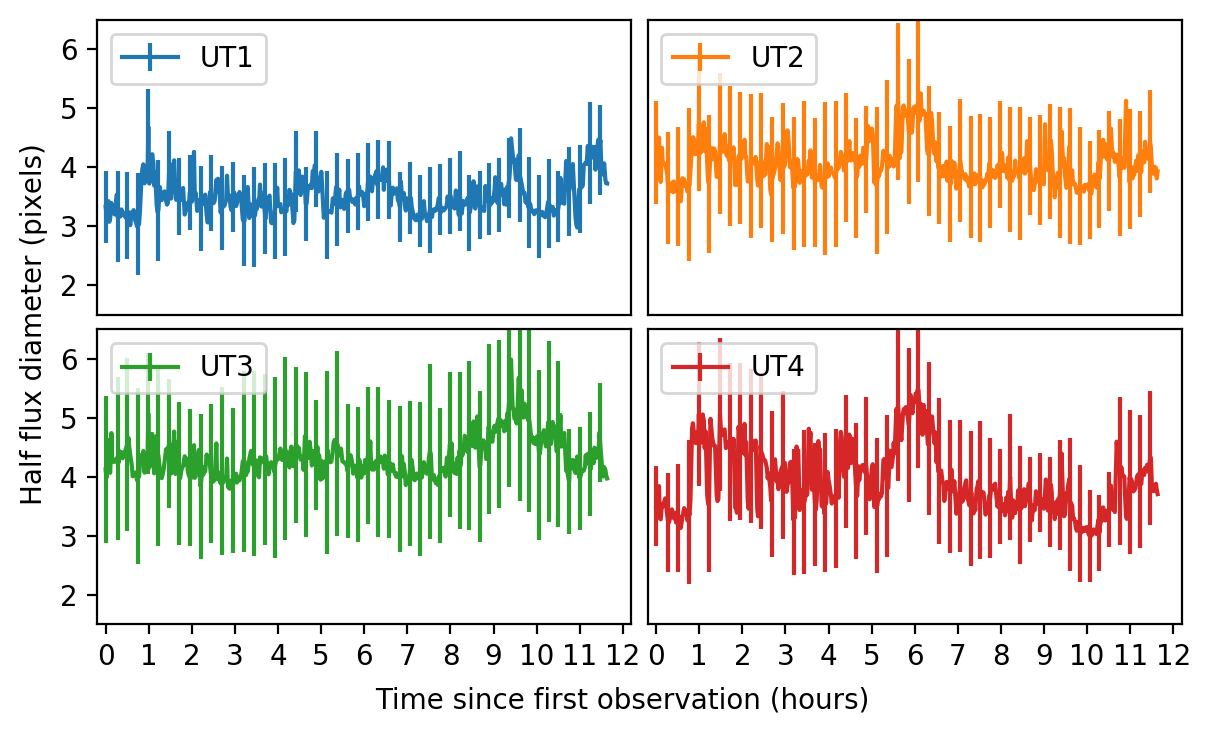
\includegraphics[width=0.95\linewidth]{images/focus.png}
    \end{center}
    \caption[Measured focus values over a night of observations]{
        Measured focus values (mean half flux diameter) over a night of observations. For clarity error bars are only plotted on every 10th point.
    }\label{fig:focus_time}
\end{figure}

\begin{figure}[p]
    \begin{center}
    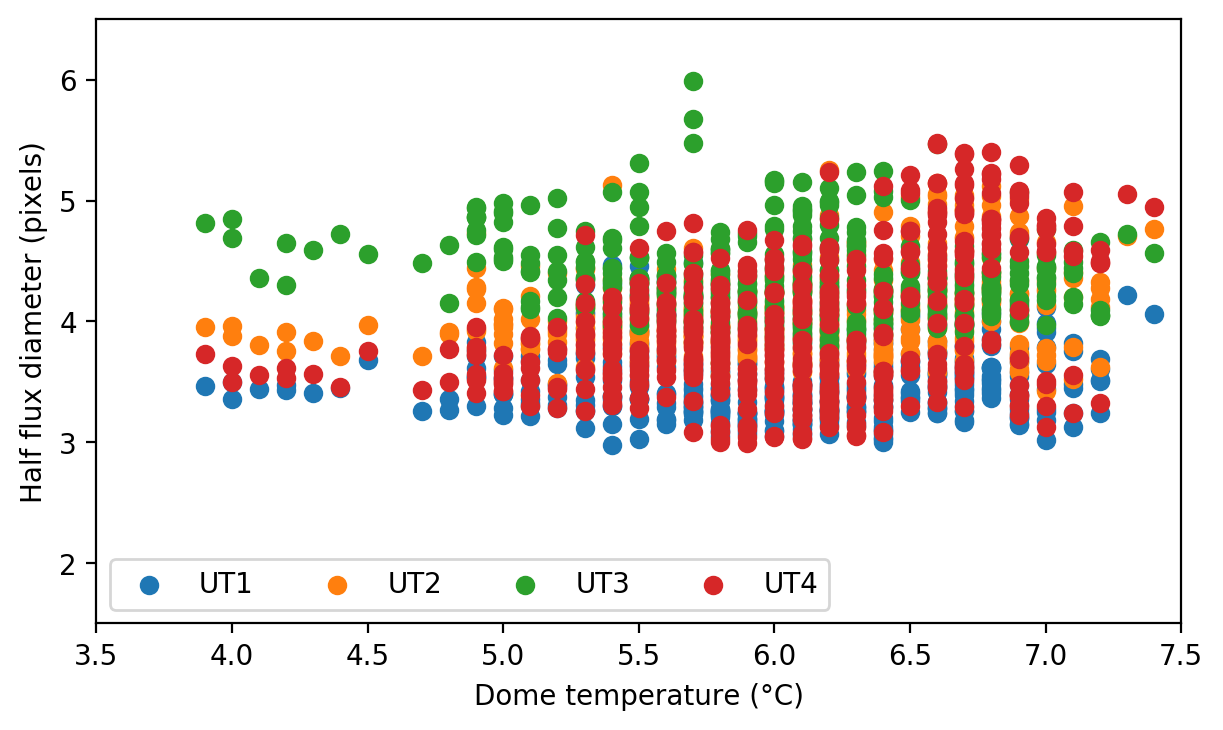
\includegraphics[width=0.95\linewidth]{images/focus_temp.png}
    \end{center}
    \caption[Measured focus values against temperature]{
        Measured focus values against temperature inside the dome.
    }\label{fig:focus_temp}
\end{figure}

\clearpage

\end{colsection}

% ~~~~~~~~~~~~~~~~~~~~

\subsection{Mount pointing and stability}
\label{sec:pointxp}
\begin{colsection}

As described in \aref{sec:mount}, using the SiTech-provided mount software (SiTechEXE) required a Windows computer for it to run on, as well as additional development effort to allow the rest of the software to interact with it. However once this was implemented it allowed us to use the various utilities built into SiTechEXE, including the pointing modelling software PointXP.\@ Using this software meant it was not necessary to create our own pointing model within the mount daemon, as once a model is created with PointXP any commands sent to SiTechEXE have the model applied before slewing.

In order to create a pointing model using PointXP the camera output from one of the telescopes needs to be connected to the Windows NUC running the software, and the rest of the G-TeCS software must be disabled to ensure PointXP has full control. The software creates a grid of equally spaced pointings at a range of altitudes and azimuths, as shown on the sky chart in \aref{fig:pointing_model}, then takes CCD images at each position, extracts the position of sources in each frame, and calculates the pointing model transformations to best convert requested coordinates to mount axis positions.

\begin{figure}[t]
    \begin{center}
        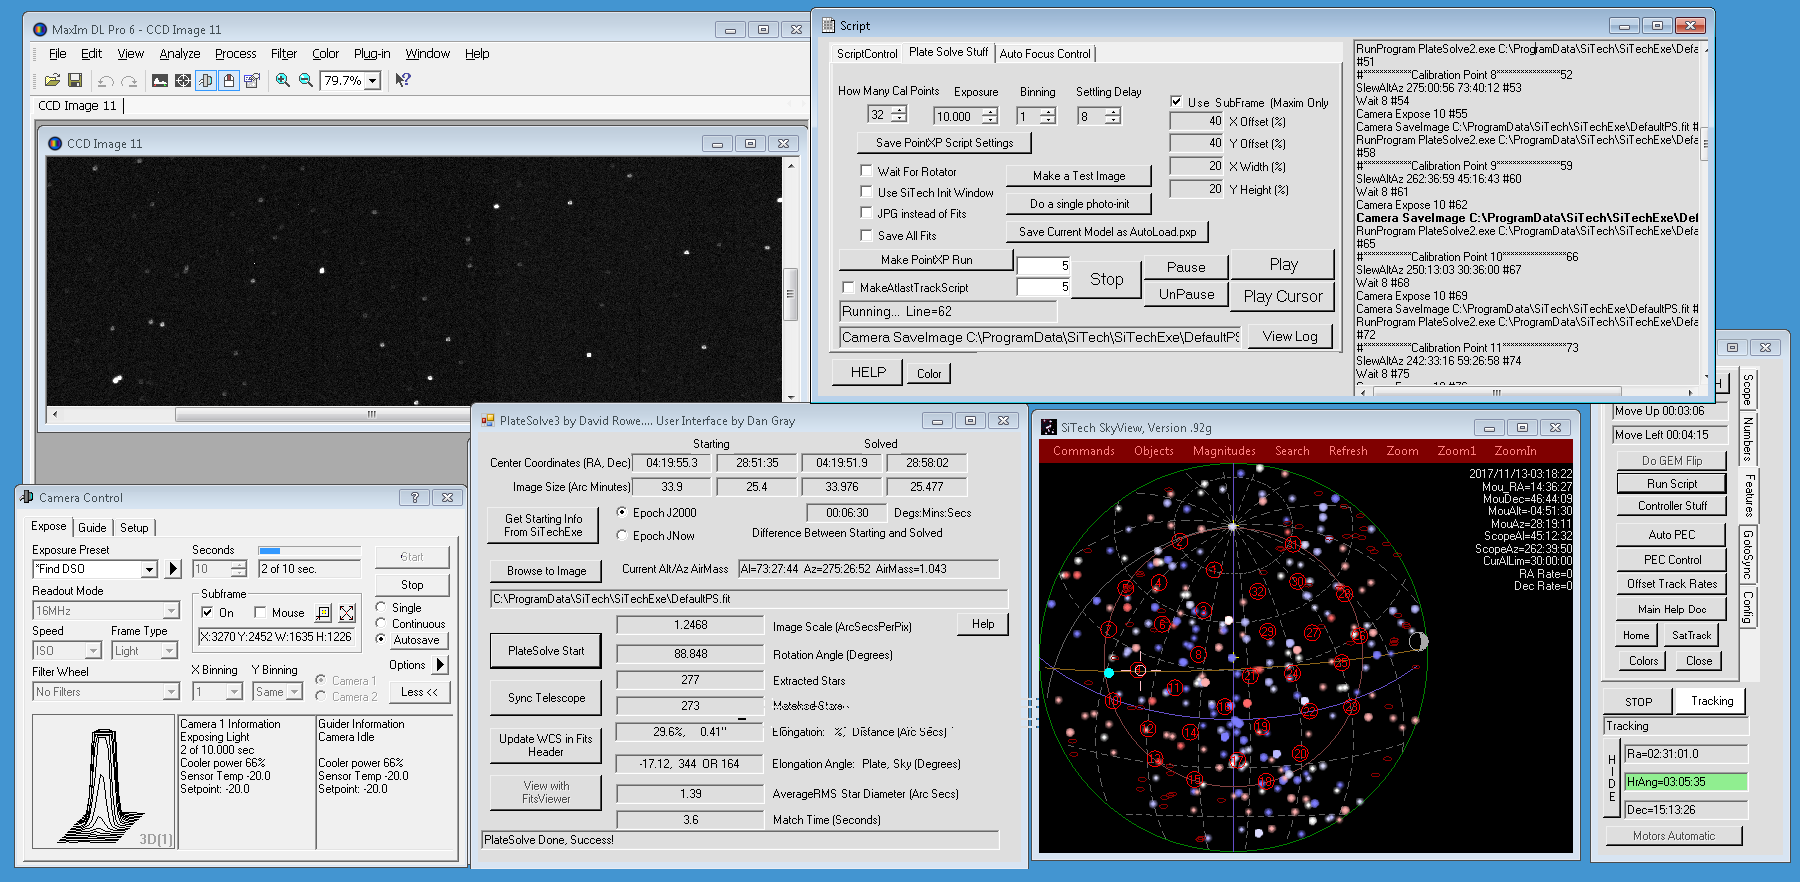
\includegraphics[width=\linewidth]{images/pointing_model.png}
    \end{center}
    \caption[Creating a pointing model using PointXP]{
        Creating a pointing model using PointXP.\@
    }\label{fig:pointing_model}
\end{figure}

One of the complications when creating a pointing model for GOTO is that the model can only be based on the output of a single unit telescope (as PointXP only expects a single camera input). When aligned into the 3-UT configuration, as shown in \aref{fig:3ut_footprint}, it was simple to create the model using the central telescope (UT4), but in the 4-UT configuration (\aref{fig:4ut_footprint}) this is not an option. The chosen camera needs to physically be disconnected from the interface NUC and connected to the Windows mount NUC PointXP is running on, which prevents creating a pointing model unless there is someone on-site. One suggestion has been to add a small guide telescope in the centre of the array which could be permanently connected to the Windows NUC PointXP is on, this could then be used to base the pointing model on.

\begin{figure}[t]
    \begin{center}
        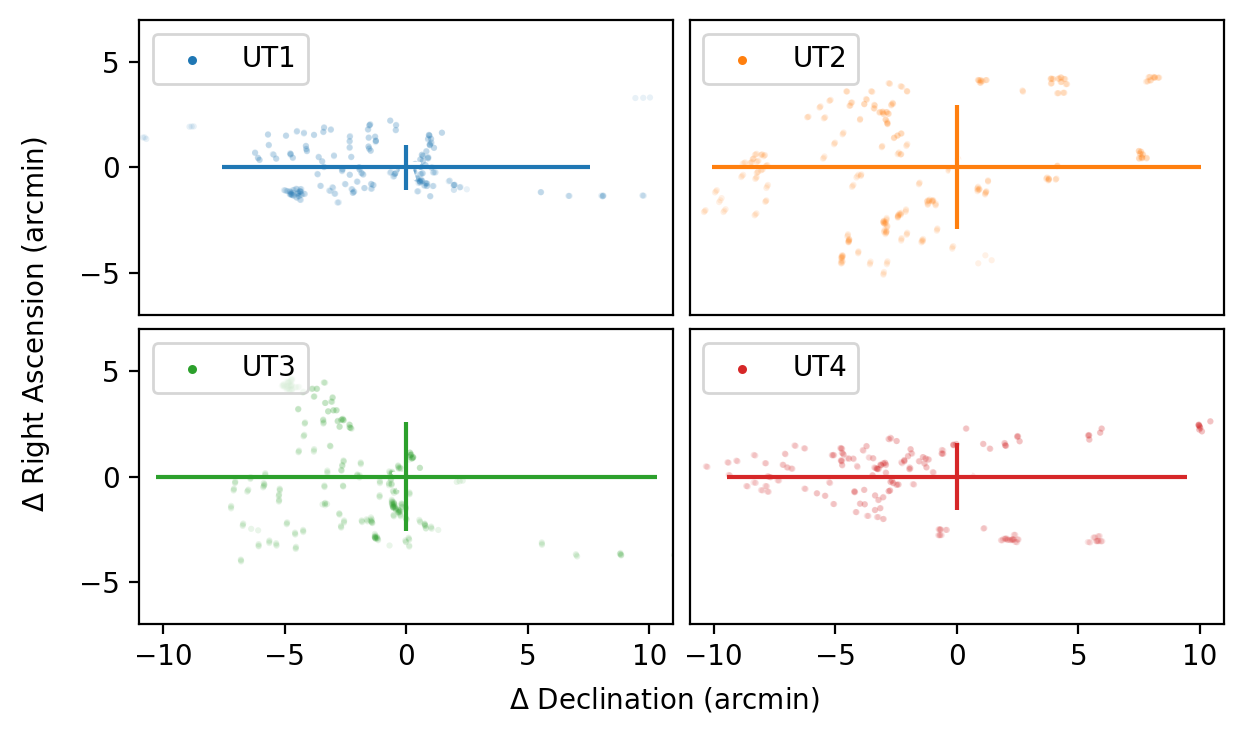
\includegraphics[width=\linewidth]{images/pointing.png}
    \end{center}
    \caption[Pointing errors over a single night]{
        Pointing errors (the difference between the target and actual image positions) taken from a single night of observations, 489 exposures in total. The error bars for each UT show the standard deviation of points in each axis.
    }\label{fig:pointing}
\end{figure}

\begin{figure}[t]
    \begin{center}
        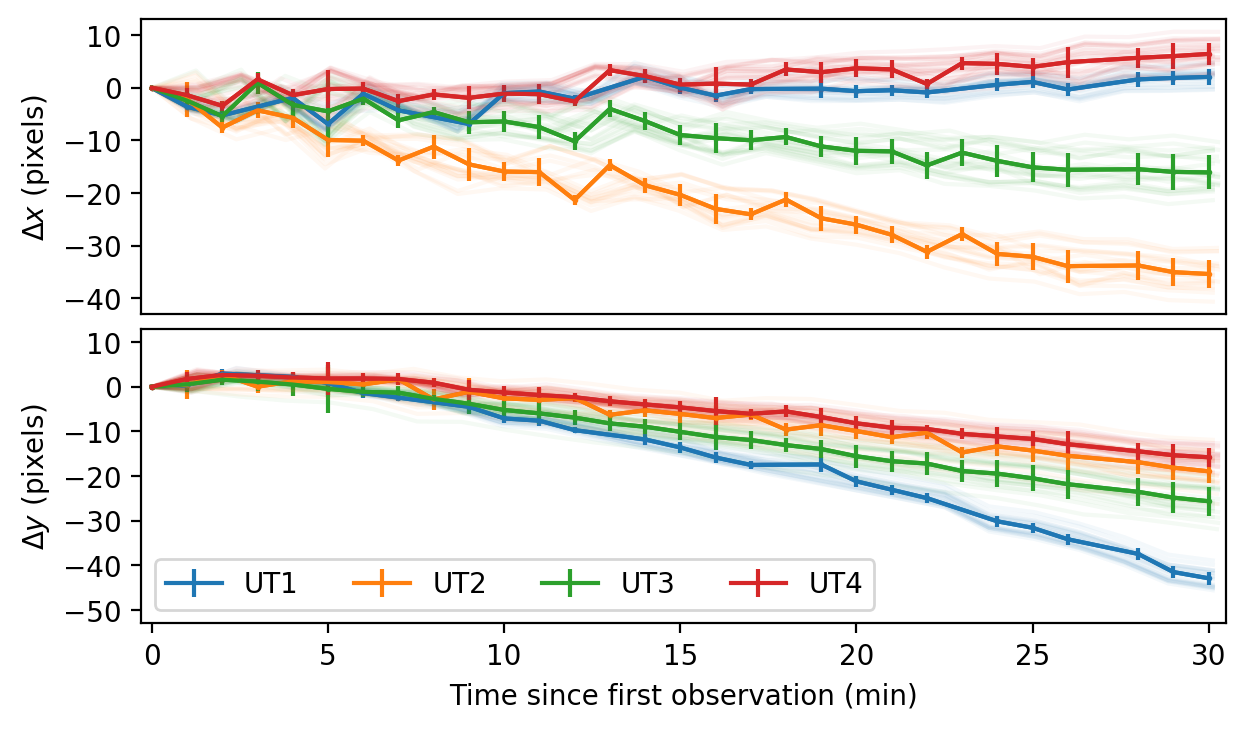
\includegraphics[width=\linewidth]{images/tracking.png}
    \end{center}
    \caption[Position drift over a 30 minute observation]{
        Position drift of sources in a series of images taken over 30 minutes. The darker solid lines show the average of all the sources detected in each UT.\
    }\label{fig:tracking}
\end{figure}

\aref{fig:pointing} shows the pointing error for each unit telescope from all images taken in a single night of normal observations after creating a new pointing model with PointXP, at various different altitudes and azimuths. The error is found as the difference between the target position reported by the mount and the actual image centre found by the GOTOphoto pipeline. As each UT has a unique offset each subplot is centred on the mean offset for that UT.\ The pointing errors vary between 8--\SI{10}{\arcmin} in right ascension and 1--\SI{3}{\arcmin} in declination, with clear variations between the unit telescopes. The pattern of points for each unit telescope also appears to be unconnected. This illustrates one of the major complications due to the GOTO mount design: each unit telescope will flex and shift slightly on their own mounts attaching them to the boom arm, in addition to the pointing of the overall mount. The original brackets mounting the unit telescopes to the boom arm were much worse and occasionally allowed unit telescopes to drift several degrees from their original position. These were replaced in July 2018, and since then the models created using PointXP have been perfectly good for use with GOTO.\@ In practice even being a few arcminutes off the desired pointing is minor compared to GOTO's large field of view, and can easily be accounted for when the images are processed by the GOTOphoto pipeline.

GOTO does not include an autoguiding system, although the proposed guide scope mentioned above could be used as one. In the absence of this the telescope must be able to track accurately. The initial mount drives suffered from tracking problems, and were very sensitive to any imbalances in the weight distribution. The motors were replaced in November 2017, and since then have been much more reliable, although it is still important to ensure that the mount is balanced. \aref{fig:tracking} shows the drift of sources taken from a series of exposures of the same target over 30 minutes, revealing a maximum drift of approximately 80 pixels/hour, or \SI{1.65}{\arcmin} (using the plate scale of \SI[per-mode=symbol]{1.24}{\arcsec\per\pixel}). Again each unit telescope has a slightly different drift in different directions (for example UT1 is very stable in the $x$ direction (right ascension) but has the biggest drift in $y$ (declination)). In practice GOTO usually switches targets every few minutes, so the long-term tracking performance over several hours is not a major concern. GOTO also typically only takes \SI{60}{\second} exposures, and no significant trailing is seen in these images.

\end{colsection}

% ~~~~~~~~~~~~~~~~~~~~

\subsection{Other commissioning challenges}
\label{sec:challenges}
\begin{colsection}

In this section I outline a few of the changes that had to be made to the software based on experience with the hardware. This is not an exhaustive list, but gives some examples of the challenges that are typical when commissioning a facility such as GOTO.\@

% ---------
\subsubsection{Filter wheel serial numbers}

One of the hardware issues that was identified early on concerned identifying the filter wheels when they were connected to the interface NUCs. The usual way to connect to specific hardware units through the FLI-API code is to search the connected USB devices for their unique FLI serial numbers (for example the serial numbers of the GOTO cameras given in \aref{tab:cameras}). However, the initial set of CFW9--5 filter wheels delivered to us by FLI did not have serial numbers defined in their firmware. Two filter wheels are connected to each interface NUC, and this problem made it impossible to tell between them or send a command to a particular filter wheel.

A solution was eventually found using the pyudev Python package (\pkg{pyudev}\footnote{\url{https://pyudev.readthedocs.io}}), which uses the Linux udev device manager to identify devices using the \code{/dev/} name, and therefore create a pseudo-serial number based on which port each device is connected to. Using this method it is possible to tell filter wheels apart as long as which physical USB port each is plugged into is known. This is not an ideal solution, but as long as the USB cables remain connected it is not an issue even if the NUCs are rebooted.

% ---------
\subsubsection{Downloading images from the cameras}

One of the more complicated parts of the camera control software is reading images from the FLI cameras. Once an exposure has finished, photo-electrons from the CCD are read out and stored as counts in a memory buffer on the camera, where they can be downloaded by USB.\@ A last-minute change led to the GOTO cameras using new, larger detectors than originally designed for the cameras, which led to there not being enough space in the camera buffer to store a full-frame image. This was discovered when corrupted images such as the one shown in \aref{fig:cam_readout} were being produced; the regions in the lower third of the image are just duplicates of the data in the upper third, meaning the original data in this section was lost.

The cameras return a \code{DataReady} status once the exposure has finished and the data is reading out. However, when installing G-TeCS on site it was clear that the camera daemon was not able to reliably start downloading the data from the cameras quickly enough to clear space in the internal buffer before it starts being overwritten. The solution was to add an internal image queue within the camera class, which would immediately begin downloading from the cameras as soon as they reported the exposure was finished. This means the camera data is stored within the memory on the interface NUCs, and then the camera daemon queries the interface (see \aref{sec:fli}) to download the image across the network and write it to disk.

\begin{figure}[t]
    \begin{center}
        
\includegraphics[width=0.7\linewidth]{images/cam_readout.png}
    \end{center}
    \caption[A corrupted image which was not read out fast enough]{
        An example of a corrupted image from one of the FLI MicroLine cameras which was not read out fast enough.
    }\label{fig:cam_readout}
\end{figure}

This solution did run into a few problems with a feature of the Python programming language called the \acro{gil}, which prevents multiple threads accessing the same Python object at once (the exact workings of the GIL are outside of the scope of this thesis). In short, this prevented reading out the cameras to the internal queue in parallel, which added an extra delay. Luckily, the FLI-API package was not written in standard Python (technically CPython) but in Cython, which interfaces between the FLI SDK written in C and the rest of the control system written in Python. Cython contains a GIL to maintain compatibility with CPython, however it is not required and can be disabled. Doing this allowed the cameras to be read out in parallel as intended.

\newpage

% ---------
\subsubsection{Declination axis encoder failure}

Just a few weeks after the inauguration the mount declination axis encoder failed, preventing any automated slewing in the declination axis (the telescope could still be moved manually with the hand-pad). Of the two axes this was by far the better one to fail, had the RA axis failed instead then the telescope would not have been able to track and so no observations could have been taken. Instead, the telescope could at least still take on-sky images, and commissioning the optics and the camera control software was able to continue by manually moving the mount.

However, the SiTech control software was not able to cope with the disabled declination axis, which meant that the telescope could not be operated in robotic mode. When sent a command to slew to a position, the mount would move to the correct RA but would never reach the target (as it could not move in declination) and therefore would not start tracking. Even sending commands to move only in RA (i.e.\ keeping the same declination position) did not work. The mount would reach the correct position but the declination encoder would never register reaching the target, so the slew was never registered as `complete' and the mount would not start tracking.

A workaround was therefore coded into the mount daemon: a separate thread which monitored the RA position and stopped the mount moving when the target RA coordinates were reached, regardless of the declination coordinates. This forced the SiTech slew command to reset, meaning it could start tracking. When this modification was in place GOTO was able to observe `normally', and was able to carry out a survey in a limited declination band of the sky. Had an important gravitational-wave alert come through during this period, the person on-site would have had to move the telescope to the correct declination and then manually carry out observations. Thankfully this was not needed, and, as described in \aref{sec:timeline}, once O2 ended GOTO was shut down until the motors could be replaced.

% ---------
\subsubsection{Dome movement}

The Astrohaven clamshell dome is driven by internal belts attached to the dome shutters. It is important when moving the dome not to put undue stress on these belts, as should one of them dislodge or snap there is nothing preventing the dome from falling open. As described in \aref{sec:dome}, the dome motors are deliberately moved in short bursts rather than continually when opening. This prevents the shutters being pulled down too fast, which can cause the upper shutter to fall and put excess stress on the belts.

As mentioned in \aref{sec:arduino}, the dome has also occasionally opened past its limits when the in-built switches fail to trigger, meaning the motors drive the shutters into the ground. The extra limit switches we installed provide a backup in order to cut the motors when they are triggered, and also give a method to detect when the shutters overshoot and let the dome daemon move the shutters back up.

One of the more serious hardware problems occurred a few days after I left La Palma in February 2018. During freezing conditions, ice had built up on the upper dome shutter, and eventually was heavy enough to partially pull the shutter open past its limits, exposing the telescope to the elements (see \aref{fig:ice_internal}). I was able to remotely move the dome and drag the shutter closed, but a large amount of ice fell into the dome. Luckily, Vik Dhillon and Stu Littlefair were still at the observatory, along with Tom Marsh, from Warwick, and my replacement GOTO monitor, Tom Watts from Armagh. As shown in \aref{fig:ice_external}, they were able to get up the mountain to clear ice from inside and outside the dome, as well as place a tarpaulin over the telescope.

Once informed about the event, Astrohaven manufactured brackets to fit inside the dome to prevent the upper shutter from being forced open in this way. The dome falling open was accompanied by a sharp drop in the internal temperature, which was the motivation to add the \code{internal} and \code{ice} flags into the conditions monitor (see \aref{sec:conditions}), to alert us should similar conditions occur in the future.

\begin{figure}[p]
    \begin{center}
        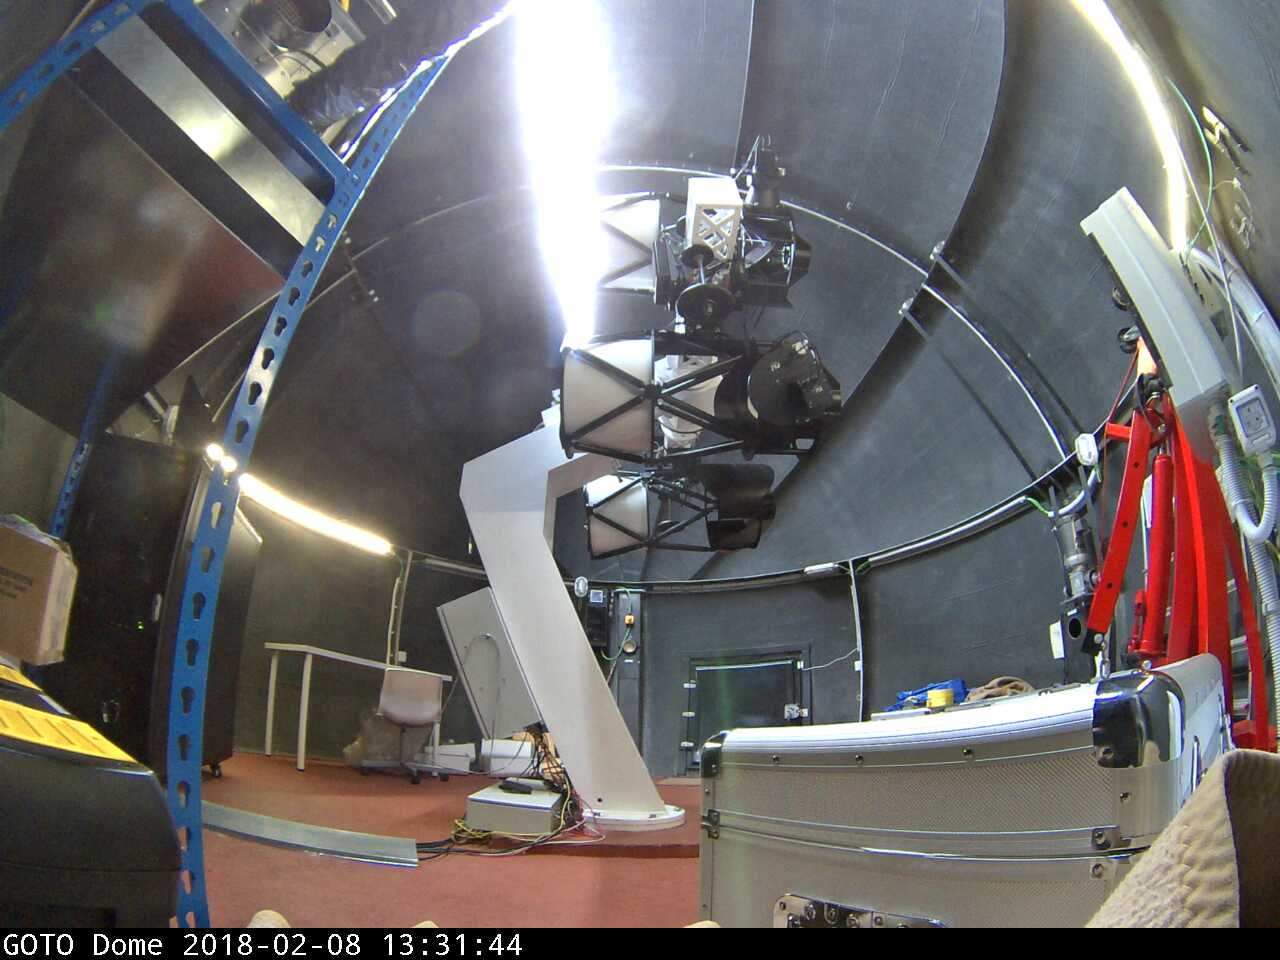
\includegraphics[width=0.45\linewidth]{images/ice_open.jpeg}
        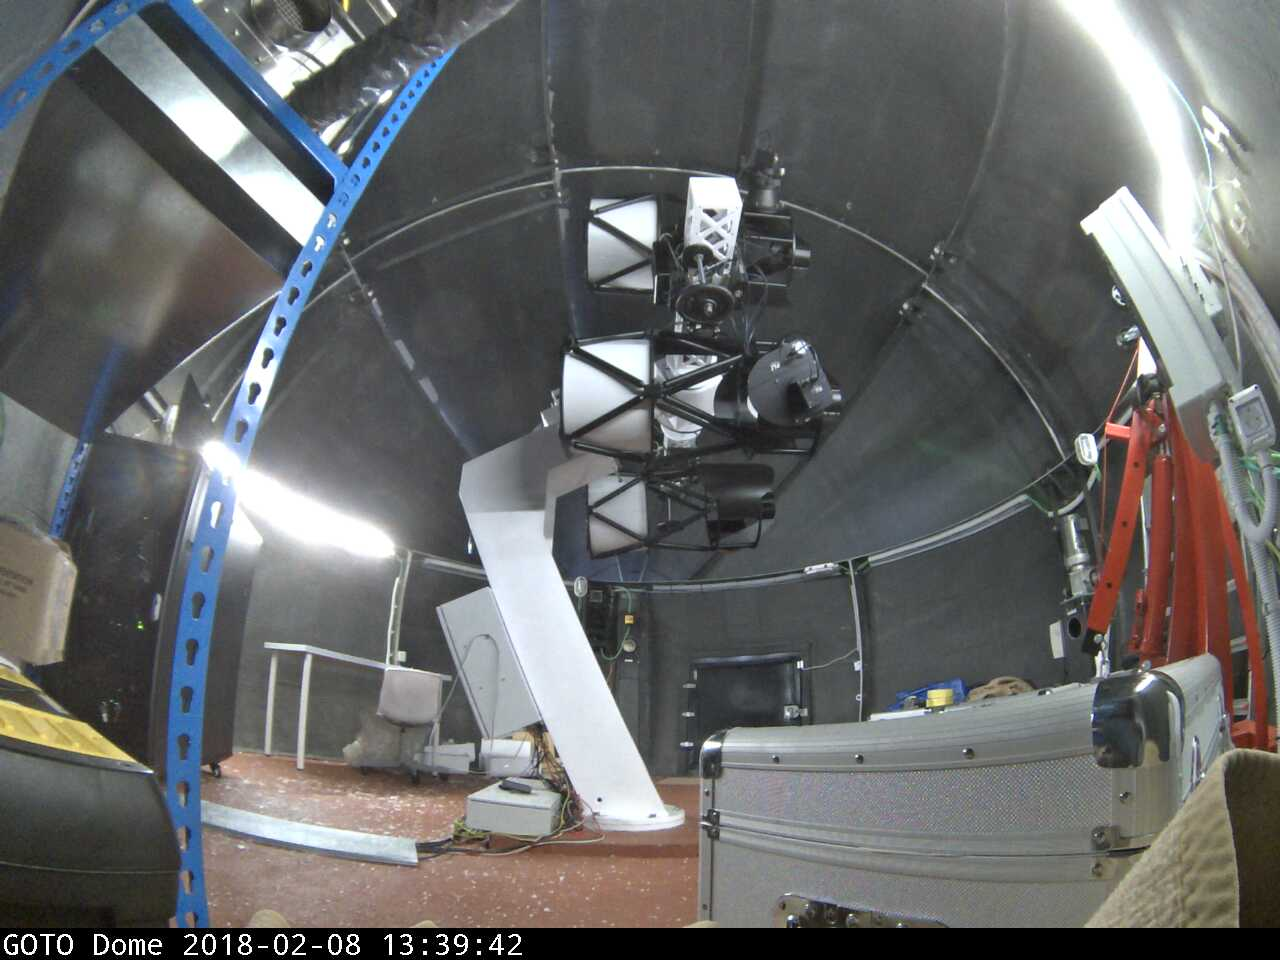
\includegraphics[width=0.45\linewidth]{images/ice_closed.jpeg}
    \end{center}
    \caption[Internal webcam images showing the dome open during a snowstorm]{
        Internal webcam images showing the dome open during the 2018 snowstorm. The image on the left was taken when opening was discovered, with the upper shutter (which normally closes on the south side, to the left of the image) having been open by the weight of ice built up on the north side. The image on the right was taken after closing the shutter remotely. Moving the dome caused a large amount of ice to dislodge and fall into the dome, thankfully missing the mirrors and camera hardware.
    }\label{fig:ice_internal}
\end{figure}

\begin{figure}[p]
    \begin{center}
    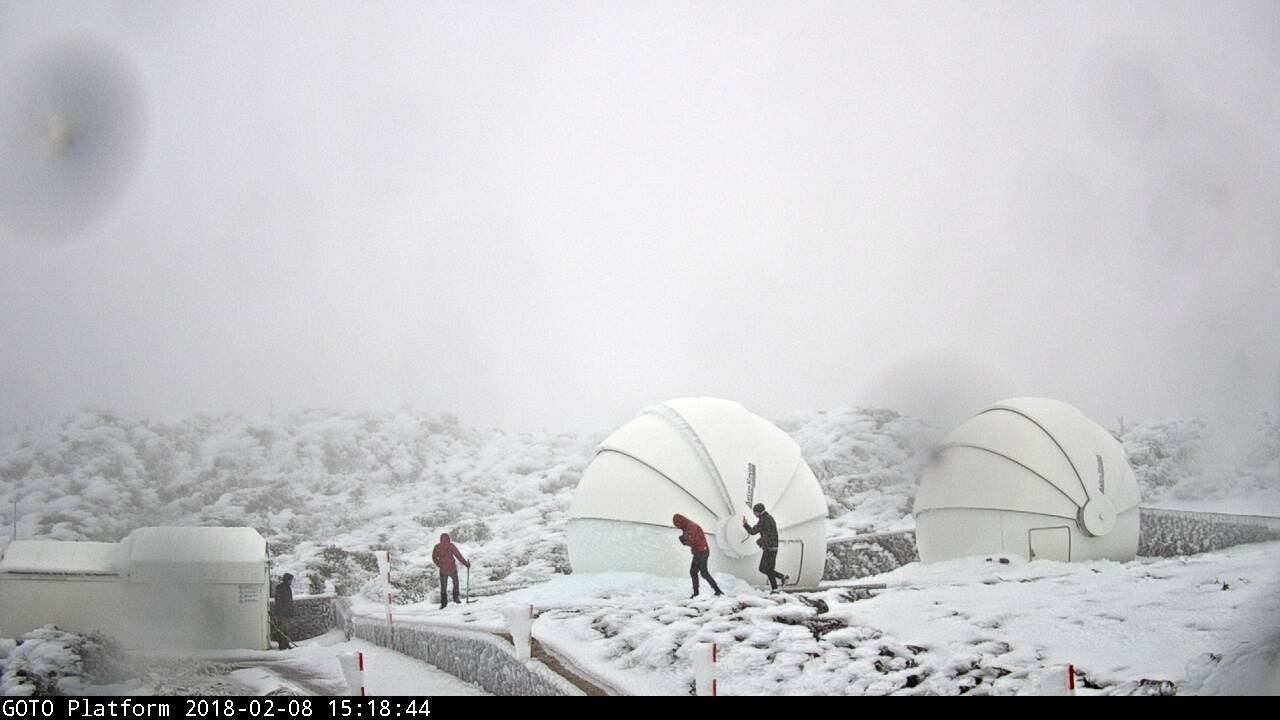
\includegraphics[width=0.88\linewidth]{images/ice_outside.jpeg}
    \end{center}
    \caption[External webcam image showing the ice rescue team]{
        External webcam image showing the ice rescue team. Note the build up of ice visible on the northern side of the upper shutter of the (empty) left-hand dome. A similar build up caused the upper shutter on the right-hand dome containing GOTO to be pulled open.
    }\label{fig:ice_external}
\end{figure}

\clearpage

% ---------
\subsubsection{Errors processing GW alerts}

Ensuring the stability of the GOTO-alert event handling system described in \aref{chap:alerts} was a high priority when commissioning the GOTO software in the run-up to the third LIGO-Virgo observing run (O3). The LVC began producing test GCN notices in December 2018 prior to the beginning of the run, which included mock skymaps similar to the ones used for the simulations in \aref{sec:scheduler_sims} and \aref{sec:gw_sims}. These events allowed a full system test of the GOTO-alert code, from the VOEvent being received to the pointings being added to the observation database.

Since the start of O3 in April 2019 until the end of August there were 32 gravitational-wave alerts, of which seven were ultimately retracted, and the G-TeCS sentinel (see \aref{sec:sentinel}) received each event and processed it using the GOTO-alert event handler code. A full run-down of the response to each event is given in \aref{sec:gw_results}. A few complications did arise during O3 which required changes to the software, mostly due to problems at the LVC's end. These are outlined below.

\begin{itemize}
    \item Initially each notice sent out by the LVC had to be approved manually by a LIGO-Virgo member, which lead to some delays to follow-up observations being triggered. The initial alert for S190421ar was delayed until several hours after the event, even though the skymap had already been uploaded by the LVC to the GraceDB service. A possible addition to the G-TeCS sentinel was proposed, a separate thread that could query GraceDB to check for new skymaps. If it detected on the skymap could quickly be processed to start GOTO observing, even before the ``official'' notice was sent out. However, since the first few events the delay between the gravitational-wave detection and the notice being sent out has been much shorter, and this modification was never implemented.
    \item An updated skymap for the S190426c event was uploaded to GraceDB by the LVC with the wrong permissions, causing the sentinel to raise an error when it could not download it from the URL in the notice. Unfortunately the event handler (see \aref{sec:event_handler}) had already deleted the existing pointings from the observation database before crashing, preventing GOTO from observing the previous tiles. After this event the order of functions in the event handler was changed, so that existing pointings were only removed once the new skymap had been downloaded and processed.
    \item The second skymap for the S190521g event was initially uploaded in an uncommon HEALPix format (see \aref{sec:healpix}) used internally in the LVC, which could not be read by GOTO-tile. Due to the above changes made following the S190426c event this did not interrupt GOTO observations, and the LVC have since clarified their filetypes.
    \item Finally, the updated skymap for the S190814bv event was incorrectly uploaded by the LVC to GraceDB with the same filename (\code{bayestar.fits.gz}) as the initial skymap (typically updates are called \code{bayestar1.fits.gz}, etc). By default, the Astropy FITS download function used within the sentinel caches each file, and if asked to download a file from the same URL will instead use the cached version. This lead to GOTO continuing to observe the large initial skymap instead of focusing on the smaller region given in the updated map. Again, the LVC have said that this will be prevented in the future, but just in case the sentinel was patched to disable the caching feature.
\end{itemize}

\end{colsection}

% ########################################

\section{Summary and Conclusions}
\label{sec:commissioning_conclusion}

% ~~~~~~~~~~~~~~~~~~~~

\begin{colsection}

In this chapter I described work carried out during the GOTO commissioning period on La Palma.

The GOTO prototype suffered several delays before finally being deployed in the summer of 2017. After that a series of hardware issues and failures lead to several elements being replaced, in particular two of the sets of mirrors. The final full prototype with four unit telescopes started reliable operations in February 2019, in time for the start of the third LIGO-Virgo observing run.

Amongst the hardware problems I installed, commissioned and developed the control software as described in the previous chapters. The primary G-TeCS hardware control systems (\aref{chap:gtecs}) were primarily developed before and during the delay in deployment, in particular I built and integrated several hardware units in the dome to ensure the safety of the telescope and any operators on site. The rest of the commissioning period was focused on developing the autonomous systems (\aref{chap:autonomous}), until in May 2018 the telescope was trusted to operate entirely robotically without full-time supervision. The G-TeCS software has proven itself to be reliable, and should provide a framework to build upon as GOTO expands.

\end{colsection}

% ########################################
